\documentclass[twocolumn]{article}

\usepackage{mathtools}
\usepackage{amsmath,amsfonts}
\usepackage{lscape}
\usepackage{bm}
\usepackage{breqn}
\usepackage{hyperref}
\usepackage{rotating}
\usepackage{pseudocode}
\usepackage{pdfpages}

\usepackage{graphicx}
\usepackage[utf8]{inputenc}

\usepackage{tikz}
\usetikzlibrary{shapes.geometric,calc}
\usetikzlibrary{patterns}

\usepackage[square,sort,comma,numbers]{natbib}

\tikzset{
	pro/.style={circle,draw=black,fill=none,inner sep=1pt,minimum size=1.3em},
	sil/.style={circle,draw=none,fill=black,inner sep=0pt,minimum size=5pt}
}

\DeclareBoldMathCommand{\t}{t}
\DeclareMathOperator{\loss}{\ell}
\newcommand{\segs}{\mathbb S}
\newcommand{\head}{\mathcal H}
\newcommand{\tail}{\mathcal T}
\newcommand{\best}{\mathcal V}

\usepackage{multirow}
\usepackage{array}
\usepackage{colortbl}

\newcommand{\sign}{\mathop{\mathrm{sign}}}

\newlength\epaisLigne
\newcommand\Mline[2]{\noalign{\global\epaisLigne\arrayrulewidth\global\arrayrulewidth#1pt}\cline{#2}\noalign{\global\arrayrulewidth\epaisLigne}}

%\newcommand{\mynote}[1]{\marginpar{\tiny #1}}
\newcommand{\mynote}[1]{}

\hypersetup{
	pdfauthor={Tim Scarfe, Wouter M. Koolen and Yuri Kalnishkan},
	pdftitle={Segmentation of electronic dance music},
	pdfkeywords={audio,stream,segmentation,dj,mixing},
	pdfsubject={Artificial Intelligence},
	pdfcreator={Tim Scarfe},
	pdfproducer={Tim Scarfe},
}

\author{Tim Scarfe, Wouter M.~Koolen and Yuri Kalnishkan \\ 
	Computer Learning Research
	Centre and Department of Computer Science, \\ 
	Royal Holloway,  University of London, Egham, Surrey, TW20 0EX, United Kingdom\\
	\{tim,wouter,yura\}@cs.rhul.ac.uk
}

\pagestyle{plain}
% to remove in the final version!!


\title{Segmentation of electronic dance music}
\begin{document}
	
	\maketitle
	
	\begin{abstract}
		
		We consider the problem of segmenting DJ-mixed dance music recordings (pod-casts, radio shows, live events) into their original sequence of contiguous tracks. We present an algorithm to reconstruct a fixed number of segment boundaries as close as possible to what a human domain expert would create in respect of the same task. As the number of segments is known in advance we do not have to rely on local points-of-change heuristics prevalent in common segmentation algorithms. We also adapt the method to estimate the number of tracks in a recording and compare our method with others. The goal of DJ-mixing is to render track boundaries invisible from human perception.
		
		Segmentation is performed on a self-similarity matrix which is derived from normalized cosines of various cost matrices which have themselves been derived from a time-series of Fourier based spectral features. The cost matrices introduced in this paper introduce notions of self-similarity, symmetry, contiguity and evolution in respect of time. 
		
		Our work incorporates self-similarity over a soft time horizon with a fixed upper boundary and is quantitatively assessed on a large corpus of radio show recordings which have been hand-labelled by a domain expert. The method could be used on other segmentation tasks and other domains. 
		\smallskip
		
		\noindent \textbf{Keywords.} \noindent music,~segmentation,~DJ,~mix,~dynamic programming
		
	\end{abstract}
	
	
	\vspace{1em}
	
	\section{Introduction}
	
	Electronic Dance Music tracks are usually mixed by a disc jockey (DJ). For this reason EDM music streams are unique compared to other genres of music. Mixing is the \textit{modus operandi} in electronic music. We first transform the audio file into a time series of features discretized into adjacent tiles and transform them into a domain where pairs from the same track would be distinguishable by their cosine. Our features are based on a Fourier transformation with convolution filtering to accentuate prominent instruments and self-similarity within tracks. We create a similarity matrix from these cosines and then derive cost matrices showing the costs of fitting a track at a given time with a given length. We use Dynamic Programming to create the cost matrices and again to perform the most economical segmentation of the cost matrices to fit a predetermined number of tracks. Dynamic programming means solutions to a problem are described in terms of overlapping sub-solutions to achieve a significant improvement in time complexity and therefore execution time. 
	
	Contiguous-segmentation differs from the standard clustering problem in that the clusters arrive sequentially and are contiguous (AAABBBCCCDDD, not AAABBBCCCBBB). In the literature this may also be known as \textit{time-dependent} clustering \citep{radu}. For brevity we will use the term \textit{segmentation} from now on to describe this methodology. 
	
	Our work mainly considers a segmentation that is globally-optimised and based upon the number and self-similarity of segments, avoiding transient points-of-change methods. Music and mixes of music have the property that they are made up of recursively repeating self-similar regions. Our method does not strictly require any training or tenuous heuristics to perform well. The distinguishing feature of our problem domain is that the number of segments is known a priori but the segmentation boundaries are not known, or ambiguous and subjective. However, computing the best solution is desirable.
	
	The intended purpose of the algorithm is to reconstruct optimal boundaries given a fixed number of tracks known a priori. The track listing is usually published by the DJ so the number of tracks is known. This is relevant when one has recorded a show (perhaps automatically), downloaded a track list and needs to reconstruct the indices given that track list. The order of the indices reconstructed is critical so that we can align the correct track names with the reconstructed indices. 
	
	 
	 
	%TODO:
	
	We extend it to estimate the number of tracks and compare to other methods. %IN SECTION BLABLA we show that we do BLABLA
	
	One of the interesting features of audio is that you \textit{cannot scrub through it, and get an overview in the same way you can with video}. Audio has a reduced \textit{contextual continuum} when the user skips through it, perhaps due to the lack of redundant, persistent scene-setting information or indeed a psychological reason. Even in video applications, discovery, context and scrubbing are an active area of research \cite{Matejka:2013:SIO:2470654.2466149}. Time index meta-data would allow click through monetisation, and allow improved use-case scenarios (for example publishing track names to social networks, information discovery and retrieval). Capturing meta-data in audio is a time consuming and error-prone process. Tzanetakis \cite{tzanetakis1999framework} found that it took users on average $2$ hours to segment $10$ minutes of audio using standard tools. While not directly relevant we might glean from those findings that there is a strong motivation to automate this process.
	
	DJs always match the speed or beats per minute (BPM) of each adjacent track during a transition and align the major percussive elements in the time domain. This is the central concept of removing any dissonance from overlapping tracks. Tracks can overlap by any amount. DJs increase adjacent track compatibility further by selecting adjacent pairs that are harmonically compatible and by applying spectral transformations (EQ).
	
	\subsection{Literature Review}
	
	Audio segmentation in the literature is colloquially implemented in the context of structural analysis. Music structure denotes the organization of a composition by its melody, harmony, timbre and rhythm. Repetitions, transformations and evolutions of music structure also contribute to its identity and it is this semantic information that structural analysis algorithms aim to extract from music. An example structure for a song might be ``Common'' $\rightarrow$ ``Verse'' $\rightarrow$ ``Chorus'' $\rightarrow$ ``Common''. Speaker diarization is another example of structural analysis 
	
	Segmentation in the context of structural analysis has been thus far been concerned with creating a novelty function to find points-of-change using distance-based metrics, rather than trying to find a fixed number of segments. Heuristics with hard decision boundaries have been used to find the best change points, for example Tzanetakis \cite{tzanetakis1999framework} used first-order derivatives of a time series of audio features. 
	
	The use of a similarity matrix to visualize and analyse local time dependencies (then called ``Recurrence Plots'') was first proposed by Eckmann\citep{eckmann1987recurrence}.
	
	J.\ Foote et al \citep{foote1999visualizing,foote1997similarity,foote2000automatic,foote2003media,foote2001visualizing} were the first to use self-similarity matrices to visualise and exploit time dependencies in music data. Foote evaluated a Gaussian `tapered' checker board kernel along the diagonal of a music self similarity matrix to create a 1-dimensional novelty function that had the notion of self-similarity over a fixed time horizon. The kernel was `tapered' down to zero on the top right and bottom left edges to reduce edge effects. The dynamic program in this paper allows any self-similarity time horizon up to a fixed limit (Foote's work had a fixed kernel size).
	
	Goodwin et al.\ used a dynamic program for segmentation \citep{goodwin2004dynamic}. Their intriguing supervised approach was to perform Linear Discriminant Analysis (LDA) on the features to transform them into a domain where segmentation boundaries would be emphasised and the feature weights normalized. Afterwards, Goodwin formulated the problem into one of finding the globally minimum cost path through a state graph (`cluster space trajectory') modelling local and transition costs. Goodwin already demonstrated in \citep{goodwin2003audio} that novelty peaks often exist within segments, not only on the boundary of segments and took the approach of modelling all possible sequential transitions between all possible clusters.
	
	A potential drawback of the approach by Goodwin and all other approaches in scene analysis segmentation that we are aware of; is that they are somewhat local methods that focus on points-of-change rather than optimizing for the best possible results for a fixed number of segments. 
	
	All contiguous segmentation algorithms that we looked at do not know a priori how many segments to find. In almost all applications, the number of known segments derives from knowledge of where boundaries are. This is the reason why the algorithm presented in this paper is unique.  
	
% no no no totally wrong, viterbi was for scene analysis 
%they used some dumb pocmethod for segmentation	Peeters et al \citep{peeters2002toward,peeters2004deriving} did some %interesting work combining k-means and a transformation of the segmentation %problem into Viterbi (a dynamic program).
	
	\citep{hauptmann1998story}
	
	% ADD HERE THAT WE ALSO USE LINDMIKS DATASET, so its the true'er' index
	A distinguishing feature of our approach is that we evaluate how well we are doing compared to humans in respect of the same task. We compare our reconstructed indices to the ones created by a human domain expert and the algorithm itself is optimised for the domain of mixed music. 
	
	% Our method is not specialised for the domain of music segmentation. It would work in other domains.. ?
	
	In the coming sections we describe the corpus (see Section~\ref{dataset}), human accuracy (see Section~\ref{human_acc}),  the evaluation criteria (see Section~\ref{eval_crit}), how we pre-process the data (see Section~\ref{proprocessing}), how we perform feature extraction (see Section~\ref{feat_ex}), designing the cost matrices using observed phenomena in the domain (see Section~\ref{costmatrix_sec}), computing the best segmentation (see Section~\ref{best_cost}), discussion of confidence intervals (see Section~\ref{sec:confidence-intervals}), our methodology (see Section~\ref{sec:methodology}), materials used (see Section~\ref{sec:materials}), results (see Section~\ref{sec:results}) and finally the summary (see Section~\ref{conclusions}).
	
	\section{Corpus}\label{dataset}
	
	We have been supplied with several broadcasts from three popular radio shows. These are: Magic Island, by Roger Shah ($106$ shows); A State of Trance with Armin Van Buuren ($109$ shows); and Trance Around The World with Above and Beyond ($88$ shows). The show genres are a mix of Progressive Trance, Uplifting Trance and Tech-Trance. 
	
	There are no silent gaps after the introduction. 
	The shows come in $44100$ samples per second, $16$ bit stereo MP3 files sampled at $192$Kbs. We resampled these to $4000$Hz $16$ bit mono (left+right channel) WAV files to allow us to process them faster. We have used the ``Sound eXchange''\footnote{\url{http://sox.sourceforge.net}}  program to do this. These shows are all $2$ hours long. The overall average track length is $5$ and a half minutes (slightly less for Magic Island (see Figure~\ref{fig:tracklengths})) and normally distributed. The average number of tracks is $23$ for ASOT and TATW, $19$ for Magic Island. There is a guest mix on the second half of each show. The guest mix DJs show off their skills with technically convoluted mixing, so it is fair to say that the boundary ``complexity'' increases during the guest mix and is at least not fixed throughout the shows.
	
	An additional dataset of $36$ radio shows have been mixed by and annotated by Mikael Lindgren (the so called \textit{lindmik} dataset). These shows are extremely useful because the DJ is the same person that created the ground truth time indices. Also there is less noise, for example voice-overs, guest mixes, radio show sounds, introductions etc. These shows also vary significantly in length from $1$ hour to nearly $5$ hours. There are $339$ shows in total.
	
	We believe this corpus is the largest of its kind used in the literature going on the comparative table of segmentation corpora listed by Peiszer et al in their literature review of audio segmentation \cite{peiszer2008automatic}. More recently Badawy et al \citep{elaudio} used a corpus of $61$ hours. The corpus we are using is longer than $680$ hours in length. 
	
	\begin{figure}
		\centering
		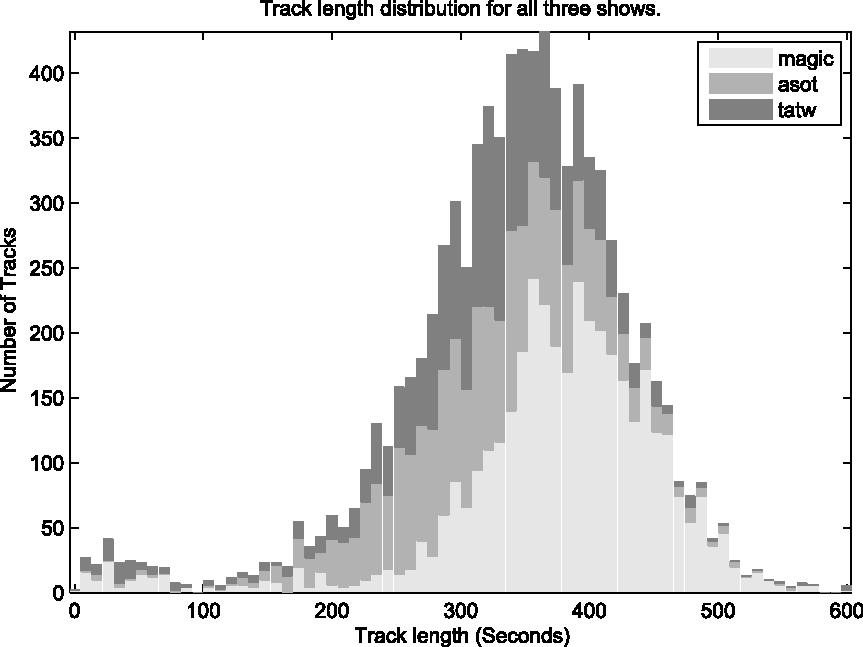
\includegraphics[width=0.45\textwidth]{images/tracklength}
		
		\caption{The track length distribution for all three radio shows. The \textit{bump} of short tracks (less than $3$ minutes) is often introductions or otherwise extraneous.}
		\label{fig:tracklengths}
	\end{figure} 
	
	There is already a large community of people interested in getting track/time meta-data for DJ sets. ``CueNation''\footnote{\url{http://www.cuenation.com}} is an example of this. CueNation is a website allowing people to submit \textit{cue-sheets} for popular DJ Mixes and radio shows. A cue-sheet is a text file containing time meta-data (indices) for a media file.
	
	The three main radio shows in the corpus were hand captured by Denis Goncharov; a domain expert and one of the principal contributors to \textit{CueNation}. One of the significant problems with this task is that there is a random error variable associated with the human captured indices themselves. On some tracks, it is unclear where to place the optimal index and when analysing our results, we have noticed some obvious human errors. Regrettably, there is no clear way of quantifying this. Many of the cue-sheet authors themselves reject the idea of automating the task, citing the poor precision of any such result (they often place indices on the exact MP3 frame). However this sentiment seems misplaced given that they frequently make mistakes or that it is a matter of opinion where to place the track and some consistent method may be preferential. A potential outcome of our method could be an assistance mechanism to help them with initial placements. Our results demonstrate that it is indeed possible to automate this task and that while there is some uncertainty attached to the optimal placement, it is still largely predictable. Indeed on the majority of track indices the uncertainty is ostensibly small. 
	
	Denis Goncharov provided us with the following description of how he captures the indices. To quote from a personal email exchange with Denis:
	
	\begin{quote}
		Trance music is made in slices of $8$ bars ($1$ bar is $4$ beats. At $135$ beats per minute, $8$ bars is $\frac{60}{135} ( 4 \cdot 8 ) \approx 14.8$ sec). Trance music tends to be around $130$-$135$ BPM. It is a matter of personal preference which point of the transition to call the index. My preference is to consider the index to be the point at which the second track becomes the focus of attention and the first track is sent to the background. Most of the time the index is the point at which the bass line ($400$Hz and lower) of the previous track is cut and the bass line of the second track is introduced. If the DJ decides to exchange the adjacent tracks gradually over the time instead of mixing them abruptly then it is up to the cue-sheet maker to listen further into the second track noting the musical qualities of both tracks and then go back and choose at which point the second track actually becomes the focus of attention.
	\end{quote}
	
	The most obvious and pervasive element in dance music is the percussion (the beats). We believe on balance that ignoring the percussive information is advantageous, because DJs use percussion primarily to blur boundaries between tracks.  We tried to capture percussive based features and found that the transitions between tracks and indeed groups of tracks appeared as stronger self-similar regions than the actual tracks. The percussive feature extractor transformed the autocorrelation of the audio samples in the time domain tiles, and compared the cosine of their absolute values. It was reasonably clear from that  research that track boundaries are revealed with less uncertainty between instruments and harmonic content. However. We do not rule out looking at percussive features again in future research because we are currently ignoring potentially useful features.
	
	Some DJs ``mix harmonically'' (by matching instruments as opposed to percussion) but this preys on human hearing and perception. An algorithm capturing the harmonic information would most likely be able to distinguish two harmonically compatible tracks. 
	
	\section{Human Accuracy}\label{human_acc}
	
	We did some analysis on how accurate the humans themselves are at creating indices. In the absence of a perfect data set our analysis instead hinged on the amount to which the humans disagreed with each other aggregated over a large amount of historical data. Mikael Lindgren was kind enough to send us a dump of his cuesheet database to experiment with. As ASOT is such a popular show there were many independently captured cuesheets to compare against for all of the historical shows. We selected all the shows having at least $3$ distinct cuesheets (not copies or shifted/misaligned copies of each other)  and such that all the cuesheets had the same number of tracks. The first track was ignored (as it was always $0$ seconds). We ended up with $115$ shows with $3$ authors. $65$ shows with $4$ authors and $30$ shows with $5$ authors.  We generated a histogram of distances from the median time for each track, for each cuesheet and assumed values greater than $100$ seconds or less than $-100$ seconds were outliers. The standard deviation of the `human disagreement' variable is $9.13$ seconds. See Figure~\ref{fig:human_muchconfuse} for an illustration. So at this stage it does not seem feasible for us to achieve a higher accuracy when we are evaluating against a method which is intrinsically error prone. An important caveat here is that ASOT turned out to be the most error-prone show to segment out of our corpus. The standard deviation of the bumps could be reduced if we normalized the times by the BPM of each transition. 
	
	\begin{figure}
		\centering
		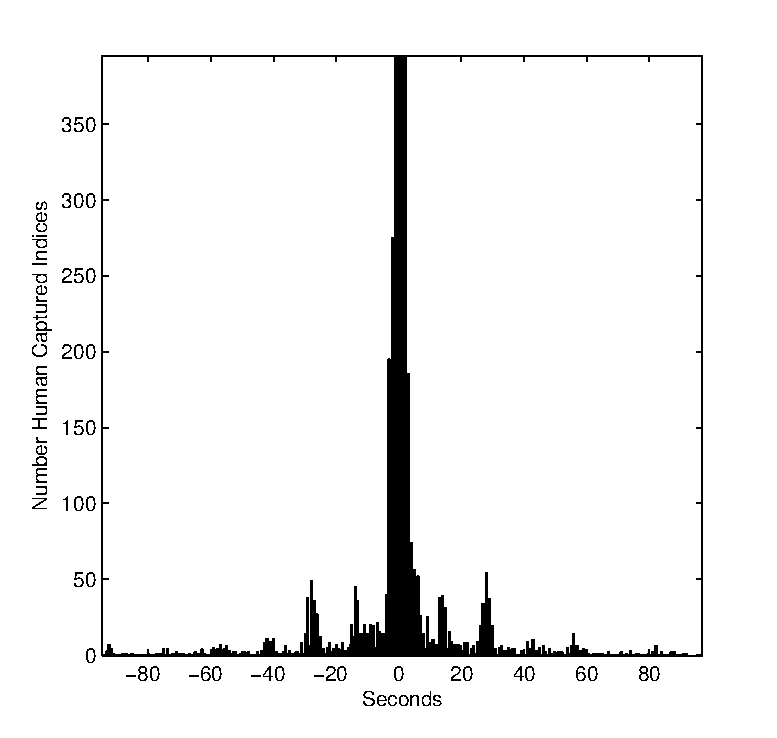
\includegraphics[width=0.45\textwidth]{images/human_confusion}
		
		\caption{Illustration of the `human disagreement' random variable (zoomed in at the bottom), standard deviation $9.13$ seconds. Peaks are visible at intervals of $8$ bars ($\approx 14.8$ seconds) which corroborates the analysis from Denis Goncharov in Section~\ref{dataset}. }
		\label{fig:human_muchconfuse}
	\end{figure} 
	
	\section{Data Handling}
	
	\subsection{Preprocessing}\label{proprocessing} % Fourier/xcorr
	
	The corpus had some outliers that may have slightly distorted the analysis of our method. Many of the ``tracks'' in our data set (of indices) were in fact not tracks at all but rather introductions or voice-overs. Almost all of these outlier tracks were short in length. These are quite clearly visible on the distribution of track lengths on Figure~\ref{fig:tracklengths}. To ameliorate the situation we removed any tracks that were shorter than $180$ seconds. We also removed any end tracks that were shorter than $240$ seconds as very often the end tracks on a radio show contain strange elements (for example voice-overs, interviews, show-related `jingles'). This required some manipulation of the cue-sheets and audio files. The undesired segments of the audio files were chopped out, and the cue-sheets were re-flowed so that the time indices point to the correct location in the file. 
	
	The algorithm still performs similarly when removing just these indices and leaving the audio intact underneath, so it would not significantly affect any real-world implementation. 
	
	For those wishing to use this algorithm in practice with pre-recorded shows; the introductions at the start of the shows are often fixed length or at least predictable so error would be small on average.
	
	The lindmik dataset which was noise-free did not require any preprocessing. 
	
	\subsection{Feature Extraction}
	
	\subsubsection{Music}\label{feat_ex} % Fourier/xcorr
	
	We used SoX (see Sect.~\ref{dataset}) to downsample the shows to $4000$Hz. We are not particularly interested in frequencies above around and above $2000$Hz because instrument harmonics become less visible in the spectrum as the frequency increases. The Nyquist theorem \cite{nyquist1928certain} states that the highest representable frequency is half the sampling rate, so this explains our reason to use $4000$Hz. We will refer to the sample rate as $R$. Let $L$ be the length of the show in samples.
	
	Fourier analysis allows one to represent a time domain process as a set of integer oscillations of trigonometric functions. We transform the tiles into the frequency domain using the discrete Fourier transform
\[
F(x_k) = X_k = \sum_{n=0}^{N-1} x_n \cdot e^{-i 2 \pi \frac{k}{N} n}
\] which transforms a sequence of complex numbers $x_0,\ldots,x_N$ into another sequence of complex numbers $X_0,\ldots,X_N$ where $$e^{-i 2 \pi \frac{k}{N} n}$$ are points on the complex unit circle. Note that the fftw algorithm \cite{frigo2004fftw} that we used to perform this computation operates significantly faster when $N$ is a power of $2$ so we zero pad the input to the next power of $2$. We denote the tile width by $M$ in seconds (an algorithm parameter). Note that
\[
N = \frac{L}{M}
\] denotes the tile size in samples (length of show in samples over the tile size). Let 
\[
T = \left\lfloor\frac{L}{\tilde{M}}\right\rfloor
\] be the total number of tiles, and \[
\tilde{M}=\frac{L}{N}
\] the tile width in samples.
Because we are passing real values into the $F(x_k)$, the second half of the result is a rotational copy of the first half.
	
	Show samples are collated into a time series $Q_i^y$ ($T \times N$) of contiguous, non-overlapping, adjacent \emph{tiles} of equal size where $i=1,2,\ldots, T$. Samples at the end of the show that do not fill a complete tile get discarded. The affect of this is increasingly negligible with decreasing tile size. Since we zero-pad $N$ to the next power of two, this also decreases the affect.
	
	As we are not always interested in the entire range of the spectrum, we use $l$ to represent a low pass filter (in Hz) and $h$ the high pass filter (in Hz). So we will capture the range from $h$ to $l$ on the first half of the result of $F$. Let $\hat{h} = \lceil~h~\cdot~\frac{{N}}{R} ~\rceil+1$ be the position of $h$ in the spectrum, and $\hat l=~\lceil~l~\cdot~\frac{{N}}{R}~\rceil+1$ be the position of $l$ in the spectrum.
	
	Let $D_e^y$ ($T \times \hat{l}-\hat{h}+1$) denote the feature matrix.
	
	For each tile $\bar{i}=1,2,\ldots,T$ we assign 
\[
D_{\bar{i}}^{1,\ldots,\hat{l}-\hat{h}+1} = \left|~F(Q_{\bar{i}}^{1,\ldots,\tilde{M}})_{\hat{h},~\hat{h}+1,~\ldots,~\hat{l} }~\right|
\]
 selecting the part of the spectrum between the high and low pass filters $h$ and $f$.  We take the absolute values of the complex result of $F(x_k)$ (defined as its distance in the complex plane from the origin using the Pythagorean theorem).
	
	To accentuate instrument harmonics we perform convolution filtering on the feature vectors in $D$, using a Gaussian first derivative filter. This works like an edge detection/transient filter but also expands the width of the transients (instrument harmonics) to ensure that feature vectors from the same song appear similar because their harmonics are aligned on any distance measure (we use the cosines). This is an issue because of the extremely high frequency resolution from having such large inputs into $F(t_i)$. For example with a tile size of $10$ seconds and a sample rate of $4000$ we have a frequency resolution of $\frac{1}{2}10 \cdot 4000 = 20$KHz. 
	
	Typically a `short-time discrete Fourier transform' is used which has smaller sized inputs (windows) into $F(t_i)$ which are usually overlapping and are multiplied by a window function, attenuating the tails to reduce spectral leakage. Usually these window functions look similar to a Gaussian, for example;  
	\[
	\mathrm{Hann}_i = 0.5 - 0.5 \cos\frac{2\pi i}{n-1}{w(i)}
	\] where $n$ is the window size
	(see \cite{tzanetakis1999multifeature} for an example). The short-time Fourier transform is relevant when increased time precision is needed as there is a frequency-time resolution trade-off with respect of the input size to $F(t_i)$. This is not a concern in this particular application as our time resolution is never required to be better than $1$ second which would still produce adequate frequency resolution.
	
	The Gaussian first derivative filter is defined as 
	$$- \frac{2 \hat{\lambda}}{\upsilon^2}  e^{-\frac{\hat{\lambda}^2}{\upsilon^2}} $$ where 
	
	$$\hat{\lambda}=\left\{~-\lfloor 2\upsilon\rfloor,\lfloor-2\upsilon+1\rfloor,\ldots, \lfloor 2 \upsilon \rfloor~\right\},$$ and $$\upsilon = b  \frac{N}{R} .$$ $b$ is the bandwidth of the filter in Hz and this is a parameter of the algorithm. After the convolution filter is applied to each feature vector in $D$, we take the absolute values and normalize on the vector lengths.  
	
	Because the application domain is well defined in this setting, we can design features that look specifically for what we are interested in (musical instruments). Typically in the literature; algorithms use an amalgam of general purpose feature extractors. For example; spectral centroid, spectral moments, pitch, harmonicity \cite{tzanetakis1999framework}. We construct a dissimilarity matrix of cosines as is common in the literature for similar applications \cite{foote1999visualizing}. The cosines are computable easily because they are the the inner products of the respective features (the features have been normalized to unit length).
	
	Let
	\[
	S_{ij} ~=~ 1-\langle D_{i}, D_{j}\rangle,
	\] define the dissimilarity matrix.
	
Then we apply some normalizing transformations. First we center $S$
around $0.5$ by raising each element to the power $2s$, where
$s=\frac{1}{T^2}\sum_{i,j=1}^TS_{ij}$. Since for $x\in [0,1]$ and
$y>0$ we have $x^y\le x$ if $y\ge 1$ and $x^y\ge x$ if $y\le 1$, the
transformation $S_{ij}\to S_{ij}^{2s}$ increases the values $S_{ij}$
whenever the mean value $s<0.5$ and decreases them whenever
$s>0.5$. Note that the transformation keeps the values $S_{ij}$ in the
interval $[0,1]$. We find this a convenient and gentle way to rescale
$S$.

Secondly we raise each value $S_{ij}$ to a power $\hat c \in
[0.5,1.5]$ and then rescale and translate them to $[0,1]$ using
$S_{i,j}\to 2S_{ij}-1$.  The parameter $\hat c$ is tuned so as to
achieve the right balance between negative \textit{incentives} and
positive \textit{disincentives} for meaningful track placement. The
distribution of values in $S$ after the transformations will have a
raised tail on left. This will become relevant when we discuss cost
matrices as some of them depend on the sign of the value in $S$.
	
	See Figure~\ref{fig:simmatrix} for an illustration of $S$ and Figure~\ref{fig:cosine_norm} for an illustration of the  normalization.
	
		\begin{figure}
			\centering
			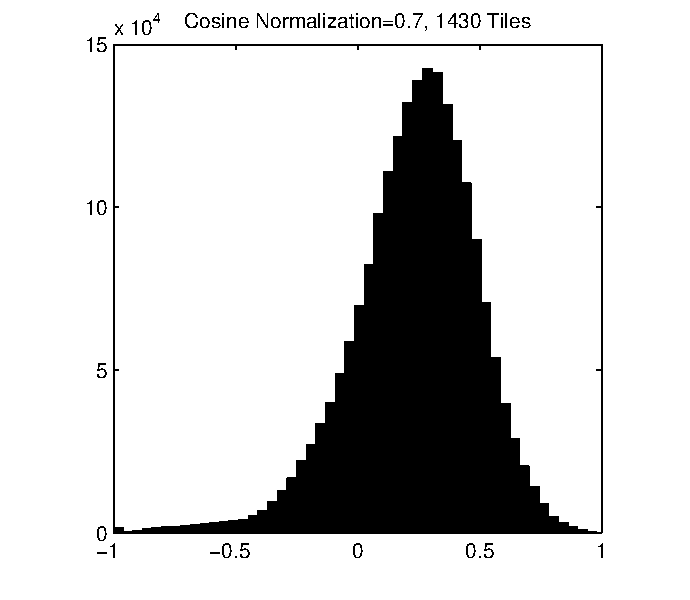
\includegraphics[width=0.45\textwidth]{images/cosinesmagic110}
			
			\caption{Illustration of the effect of normalization parameter $\hat c=0.7$ on the values in $S$ on radio show Magic Island $110$. The small raised section on the left correspond to the tracks.}
			\label{fig:cosine_norm}
		\end{figure} 
	
	\begin{figure*}[t]
		\centering
		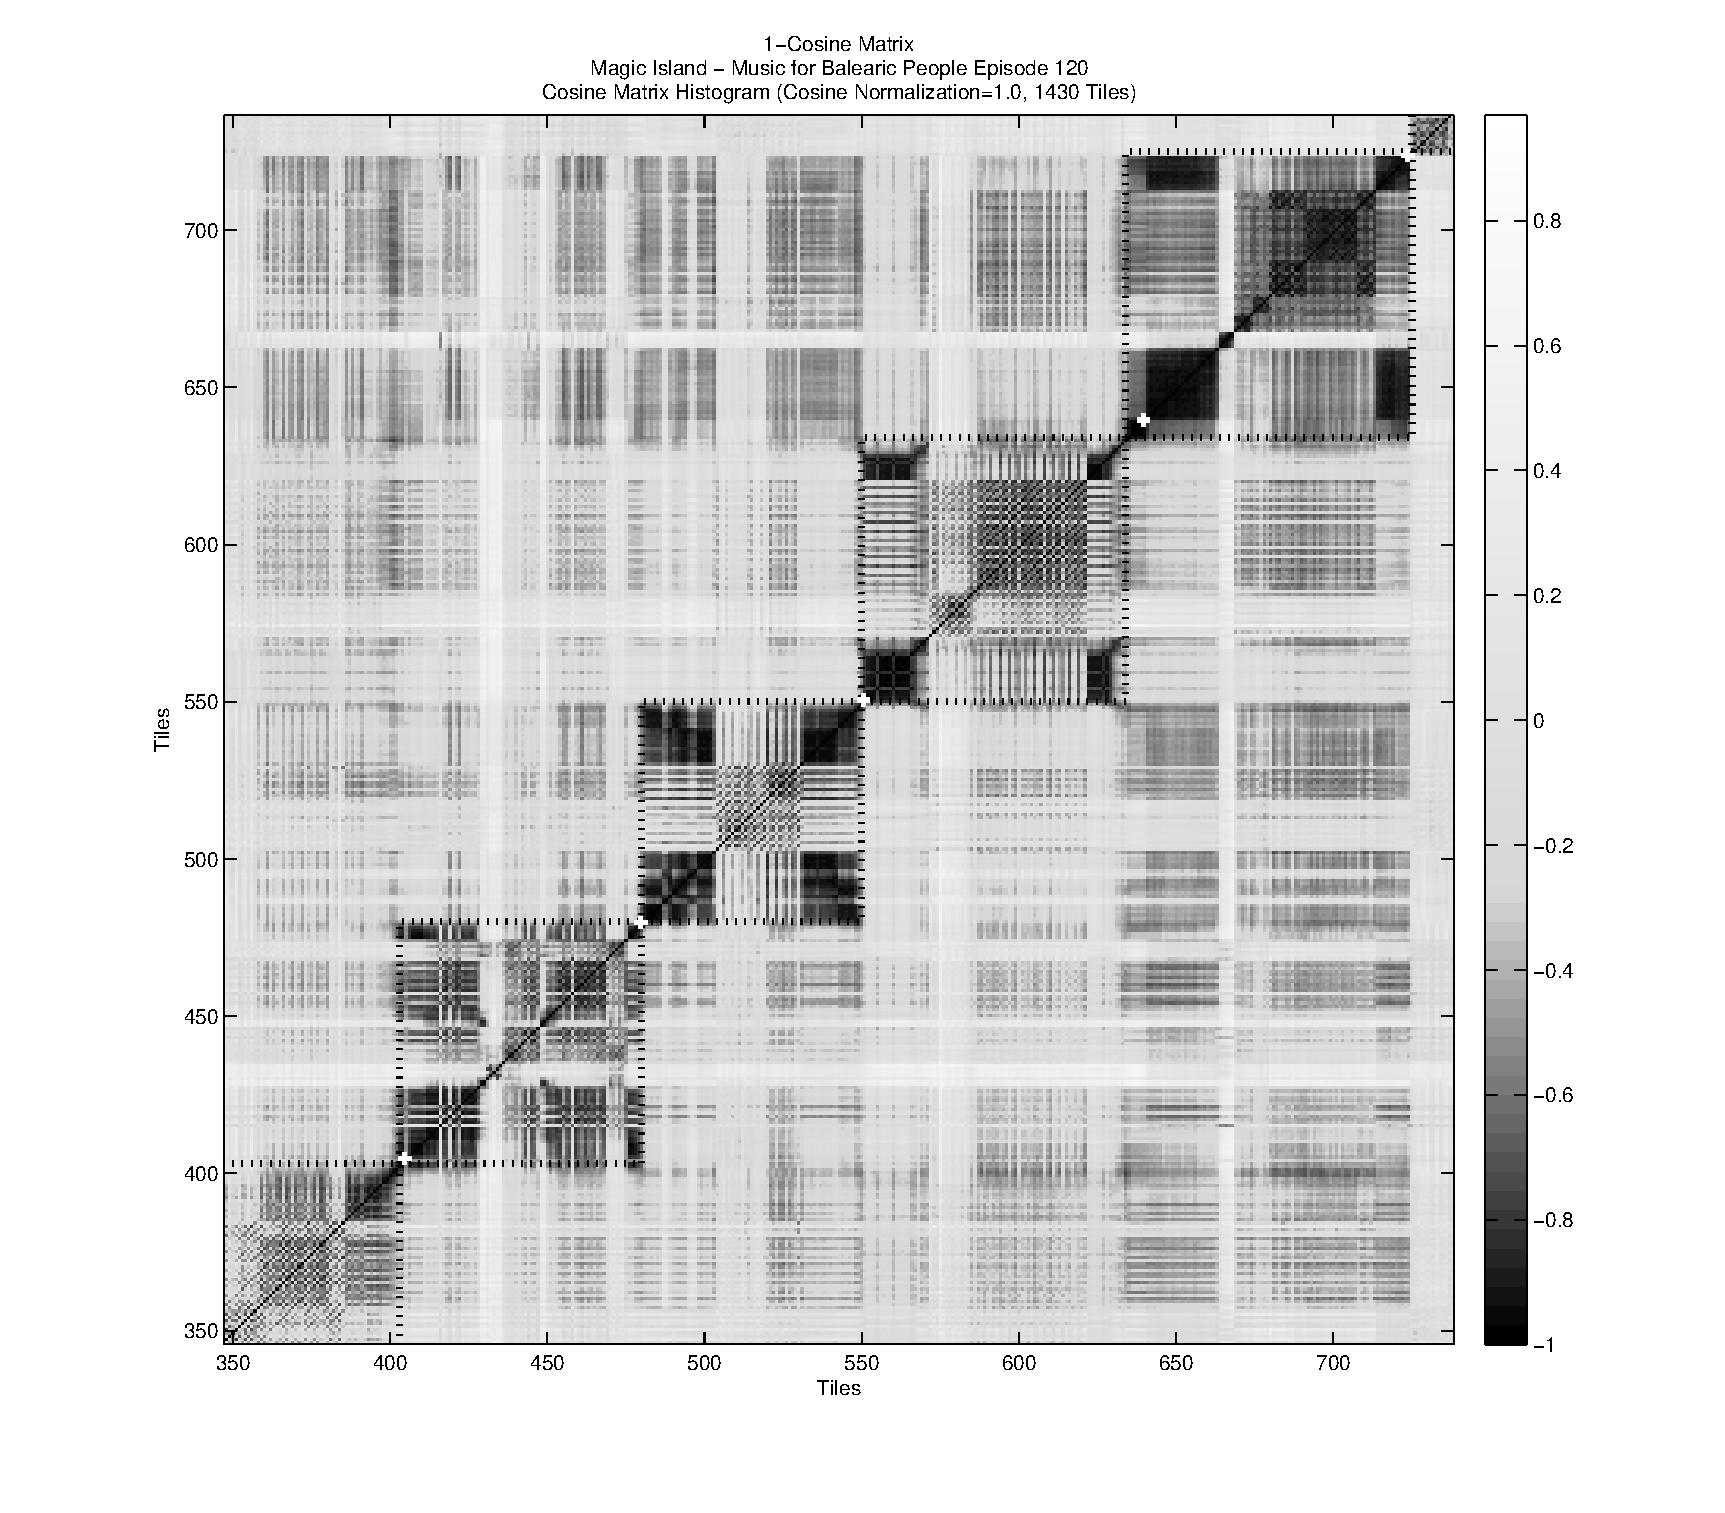
\includegraphics[width=1.08\textwidth]{images/S}
		\caption{An illustration of the similarity matrix $S$ with the actual indices drawn on with white crosses, and our reconstructed indices indicated with the black dotted lines. There are examples here of evolutionary repetition ($t=500,\ldots,550$), static contiguity everywhere where there is solid black, and symmetry on the middle two tracks.}
		\label{fig:simmatrix}
	\end{figure*} 
	
	\subsubsection{Self Similarity}\label{costmatrix_sec} % dynamic recursion
	
	We now have a similarity matrix $S_{ij}$ as described in Section~\ref{feat_ex}. 
	
	Let $w$ and $W$ denote the minimum and maximum track length in seconds, these will be parameters of the algorithm that improve the time complexity while not significantly harming the results. 
	
We proceed to constructing a cost matrix $C(f,t)$ that describes the
cost of placing a track starting at $f$ and finishing at $t$ (and
having length $t-f+1$). After analysing the data set, we have created
$7$ cost matrices that exploit observed phenomena in $S$. We also
provide an additional cost matrix which is just a Gaussian random
function centred around the mean track length for all times which can
be used to regularise the other $7$ matrices or used on its own as a
comparator to a more naive method of placement.
	
	The cost matrices exploit themes such as contiguity, symmetry, evolution and change as well as simple summation of $S$ as was presented in our last paper \citep{scarfe2013long}. In our previous work $S$ was on the interval $[0,1]$ and the summation method could only consider disincentives. The new cost matrices have a parameter to shift the consideration of incentive versus disincentive and values on the interval $[-1,1]$.
	
	On the whole, a significant number of tile pairs within one track are similar to each other. Pairs of tiles that do not belong to the same track are expected to be dissimilar, most of the time. However, tracks have contiguous regions within them that are dissimilar to each other. Transitions between songs may appear as a self-similar region but usually also similar to each adjacent track to varying degrees.  
	
	\paragraph{Summation}
	
	The most obvious strategy of all is to sum up all relevant tiles in $S$ for each candidate track from tile $f$ through tile $t$. We define $C(f,t)$, the cost of a candidate track from tile $f$ through tile $t$, to be the sum of the similarities between all pairs of tiles inside it
%it will be normalized at the end; it is easier to explain recursion without normalization

	\begin{dmath*}
		\tilde C(f,t, \Omega) =  \sum_{i,j=f}^{t} \hat S_{ij}
	\end{dmath*}
where
	\begin{dmath*}
		\hat S_{ij}=	{ \left\{
			\begin{array}{ll}
				\Omega S_{ij},  & \text{~if~}S_{ij} > 0   \\
				 \left( 1-\Omega \right) S_{ij}, & \mbox{~otherwise~}\\
			\end{array}
			\right.} 
	\end{dmath*} 
for all $i,j \in S$ (the parameter $\Omega$ control the balance of
positive and negative values). Direct computation using the definition
takes $O(TW^3)$ time. We can improve this to
$O(TW)$ by using the following recursion (assume that $f+1 \le t-1$):
	\begin{dmath*}
		\tilde C(f,t) = \tilde C(f+1,t) + \tilde C(f,t-1) - \tilde C(f+1,t-1) + \hat S_{ft} + \hat S_{tf}.
	\end{dmath*} 
The recursion implies that the cost of a track of length $L=t-f+1$ can
be calculated from the costs of shorter tracks using a constant number
of operations. The following picture (where the middle cell
corresponds to $\Upsilon = \tilde{C}(f+1,t-1)$) provides an
illustration:
	
	\begin{center}
		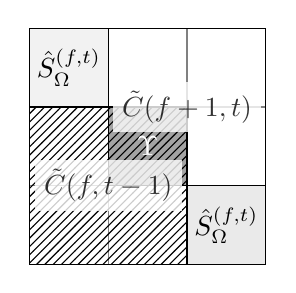
\begin{tikzpicture}
		\draw[step=1cm,color=gray] (0,0) grid (3,3);
		
		\draw[fill=gray!90, fill opacity=0.8] (1,1) -- (1,2) -- (2,2) -- (2,1) -- (1,1);
		\draw[fill=gray!10, fill opacity=1] (0,2) -- (0,3) -- (1,3) -- (1,2) -- (0,2);
		\draw[fill=black!10, fill opacity=0.8] (2,0) -- (3,0) -- (3,1) -- (2,1) -- (2,0);
		
		
	\draw [step=0.5cm, pattern=north east lines] (0,0) rectangle (2,2);
	
		
		\node[color=black] at (0.5,2.5) {$\hat S_\Omega^{(f,t)}$};
		\node[color=black] at (2.5,0.5) {$\hat S_\Omega^{(f,t)}$};
		
		
		\draw[color=black] (0,0) -- (0,2) -- (2,2) -- (2,0) -- (0,0);
		\draw[color=black] (3,3) -- (1,3) -- (1,1) -- (3,1) -- (3,3);
		
		\node[color=black,fill=white, fill opacity=0.8] at (1,1) {$\tilde{C}(f,t-1)$};
		\node[color=black,fill=white, fill opacity=0.8] at (2,2) {$\tilde{C}(f+1,t)$};
		
		\node[color=white] at (1.5,1.5) {$\Upsilon$};
		
		\end{tikzpicture}.
	\end{center} 

%	The final cost matrix is normalized by width and incentive bias
%\[
%C(f,t) \leftarrow \hat N_\Omega \left( \frac{ C(f,t) }{ t-f+1 } \right)
%\] for all $t,f \in \tilde C$.
	
	\paragraph{Symmetry}	


	
A common feature on dance music tracks is partial mirror-symmetry. We build a cost matrix to capture that.
	
Let $\Lambda(f,t,d)$ be the diagonal parallel to the minor diagonal
of $S$ and at the `distance' $d$ from it. We represent it as an ordered set
\begin{dmath*}
\Lambda(f,t,d)
 = \langle S_{f+d,f}, S_{f+d+1, f+1}, S_{f+d+2, f+2},\ldots, S_{t, t-d}\rangle.
	\end{dmath*} 
For each such diagonal in one triangle/half of $S$ we want to compare
each element against its mirror counterpart. For an ordered set
$\Lambda$ we define its cost as
\begin{dmath*}
\bar C(f,t,\Omega)(\Lambda)=\sum_{i=1}^{|\Lambda|}\delta(\Lambda_i,\Lambda_{|\Lambda|-i+1},\Omega)
\end{dmath*}
where
\begin{dmath*}
\delta(p,q,\Omega) = 
\left\{\begin{array}{ll}
0,  & \text{if~}\sign( p ) \ne \sign( q ),\\
\Omega pq,   & \text{if~}  \sign(p) \ge 0 \text{~and~} \sign(q) \ge 0 ,  \\
(1-\Omega)pq,  & \text{if~} \sign(p) < 0 \text{~and~} \sign(q) < 0, \\
\end{array}\right.
\end{dmath*}
i.e., `symmetric' pairs that have the same sign make positive
contributions and pairs that have a different sign contribute $0$ to
the cost. We define the cost matrix as
\begin{dmath*}
\tilde C(f,t,\Omega) = \sum_{d=1}^{t-f+1}\bar C(\Lambda(f,t,d,\Omega))
\end{dmath*}
Clearly, one can reuse the cost for shorter intervals to calculate the
cost of longer ones, namely, $\tilde C_{f+1,t-1}$ can be used to
calculate $\tilde C_{ft}$ this saving computation time.

	
%	Finally, the symmetry change matrix is defined where $\hat \delta$ is the same as the \textit{symmetry summation}, the width normalization is removed and the inner sum of the definition becomes the first order differences. For the sake of brevity we have omitted the dynamic programming formulations which run in $O(TW^2)$ time but they have been implemented in code and are available on-line (see Section~\ref{sec:materials}). This is also the case for all the following cost matrices.
	
	\paragraph{Static Contiguity}

% check my writing; I am not sure I understood you correctly
	
Horizontal contiguous traces in $S$ indicate that the track is
self-similar (negative values) or self-dissimilar (positive values)
due to repetition. If a given tile is the same as a set of contiguous
tiles following it, then there is some static contiguous region in the
show. The word \textit{static} denotes that the music is not evolving in
respect of time.

Let $\Gamma(f,t,h)$ be the horizontal segment in the matrix $S$
showing the similarity of tile $f+h-1$ to `future' tiles $f+h,
f+h+1,\ldots, t$. We represent is as an ordered set
\begin{dmath*}
\Gamma(f,t,h) =  \langle S_{f+h-1,f+h-1}, S_{f+h-1,f+h}, S_{f+h-1,f+h+1},\ldots,\\
S_{f+h-1,t}\rangle.
\end{dmath*} 
We define the cost of an ordered set $\Gamma=\langle
\Gamma_1,\Gamma_2,\ldots,\Gamma_{|\Gamma|}\rangle$ as
$$
\bar C(\Gamma,\Omega)=\sum_{i=\rho}^{|\Gamma|}\hat C(\Gamma^i,\Omega),
$$ 
where $\rho$ is a parameter indicating the minimum number of
contiguous tiles required, $\Gamma^i=\langle
\Gamma_1,\Gamma_2,\ldots,\Gamma_i\rangle$ and
\begin{dmath*}
\hat C(\Gamma^i,\Omega)=\\ \left\{
\begin{array}{ll}
\frac{1}{i}\sum_{j=1}^i\tilde{f}(\Gamma_j,\Omega),&
 \text{~if the numbers~} \\
& ~\sign{G_1},\ldots,\sign{G_i}\\
& \text{~are the same},\\
0, & \text{~otherwise},
\end{array}
\right.
\end{dmath*}
where
\begin{dmath*}
\tilde{f}(v,\Omega) = \left\{ 
	\begin{array}{lr}
		\Omega v, & \text{~if~} \sign v=1 \\
		(1-\Omega) v, & \mbox{~otherwise.}    \\
	\end{array}
	\right.
\end{dmath*}
The cost of an interval is defined as
\begin{dmath*}
\tilde C(f,t,\Omega) = \sum_{h=1}^{t-f}\bar C(f,t,\Omega)\enspace.
\end{dmath*}



%	We will also create a past contiguity cost matrix where we replace $\Gamma( f,t,h )$ with a version 

%\begin{align*}
%\begin{array}{ll}
%\hat{\Gamma}( f,t,h ) &= S(~\hat{i}(f, t, h), f + h - 1~),\\
%\end{array}
%\end{align*}
%where
%\begin{dmath*}
%	\hat{i}(~f, t, h~) =\\ \{~ t - h - 1, t - h, \ldots, f+h-1 ) ~\}
%\end{dmath*}

%	which traces past self-similarity from the end of the track being fitted.

Again it is possible to reuse values $\tilde C(f,t,\Omega)$ from
shorter intervals to save calculation time for longer intervals.

	
	\paragraph{Evolutionary Contiguity}

% rewrite this along the lines of what I said before.
	
	Any diagonal traces in $S$ that are parallel to the main diagonal are partial copies of the track in the future which evolve in respect of time. Evolutionary Contiguity is a cost matrix which compares all adjacent pairs on the diagonals in $\hat t$, using the comparator $\delta( p,q, \Omega )$ from the standard symmetry cost function and multiplies those values by the time horizon. All the values are summed and normalized by the track width squared. 
	
	Let the evolutionary cost matrix
	\begin{dmath*} C(f, t, \Omega) =  
		\hat N_\Omega\left(\frac{
		\sum_{d=1}^{t-f+1} 
		\sum_{i=2}^{|\Lambda( f,t,d )|}  \delta( \kappa_{i}, \kappa_{i-1}, \Omega ) \cdot d
	}{(t-f+1)^2}\right)
	\end{dmath*}  where  $\kappa_i=\Lambda( f,t,i )$. As before $\tilde C$ is normalized by track width and incentive bias.

%This formula does not make sense to me: what is raised to power 2??

	\paragraph{Gaussian}
	Let \[
	G( \varpi, N )_{tw} = e^{ - \frac{1}{2} \frac{\varpi n}{ \frac{1}{2} W}^2  }
	\] for all $n=1,2,\ldots,W$ denote the Gaussian matrix cost function of $N\times W$. $G( \varpi, N )$ is time-independent and every row is the same. We will use this cost function for regularising the others and for use on its own for comparison against a `naive' competitor. Increasing values of $\varpi$ will tighten up the Gaussian although after experimentation we observed that $1$ was always the best value and stuck with that.
	
	\paragraph{Normalization}

All cost matrices are normalized in the following manner. First we
divide $\tilde C(f,t,\Omega)$ by the track length,
$$
\tilde C(f,t,\Omega)\leftarrow \frac{\tilde C(f,t,\Omega)}{t-f+1}.
$$ 

Then we scale and shift $C$ according to the value of $\Omega$. If
$\Omega=0$, we want the resulting values to fill the interval $[0,1]$,
if $\Omega=0.5$ we want the resulting values to fill the interval $[-1,1]$,
and if $\Omega=1$ we want the resulting values to fill the interval $[-1,0]$.
For intermediate values of $\Omega$ we want a linear combination.

This is achieved by applying the normalization function to each element:
	\begin{dmath*}
		\hat N(x,\Omega) = \frac{ x - \min_{ft}C(f,t,\Omega) }{ \max_{ft} C(f,t,\Omega) - \min_{ft} C(f,t,\Omega)} \hat h_\Omega -s_\Omega,
	\end{dmath*}
where $\hat h_w$ = $2-2|0.5-\Omega|$ and
	\begin{dmath*}
		s_\Omega= { \left\{
			\begin{array}{ll}
				1-2(0.5-\Omega) & \mbox{~if~}\Omega < 0.5,   \\
				1 & \mbox{~otherwise~}.  \\
			\end{array}
			\right.}
\end{dmath*}
We let
\begin{dmath*}
C(f,t,\Omega)=N(\tilde C(f,t,\Omega),\Omega)
\end{dmath*}
for all $f$ and $t$.

	
%	Note that to save space we will use the following notation $\hat N(C, \Omega)=\hat N_\Omega(C)$.
	
	
	\paragraph{Mixing Cost Functions}
	
	We mix cost matrices together by adding them. In our experiments we will have a parameter for each cost matrix $\in [0,1]$ to show its contribution to the mixture. The cost matrices will be multiplied by this number before being mixed. 
	
	See Figure~\ref{fig:cost_matrices} for an illustration of a single cost matrix and a mixture. 

	
	
		\begin{figure}
			\centering
			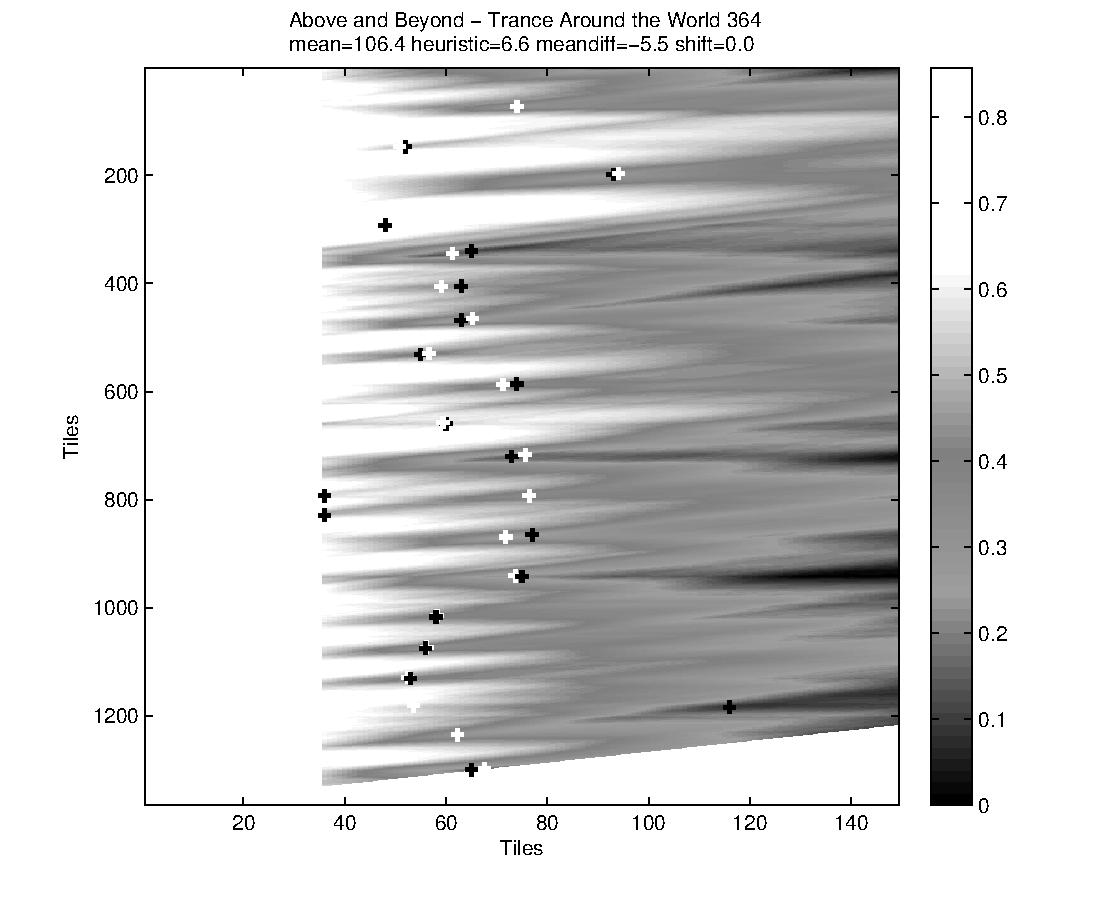
\includegraphics[width=0.45\textwidth]{images/cmsumib0}
			\caption{Summation cost matrices for Magic Island episode 110 with an incentive bias $\Omega=1$ and therefore containing disincentives. }
			\label{fig:cmsumib1}
		\end{figure} 
		
		\begin{figure}
			\centering
			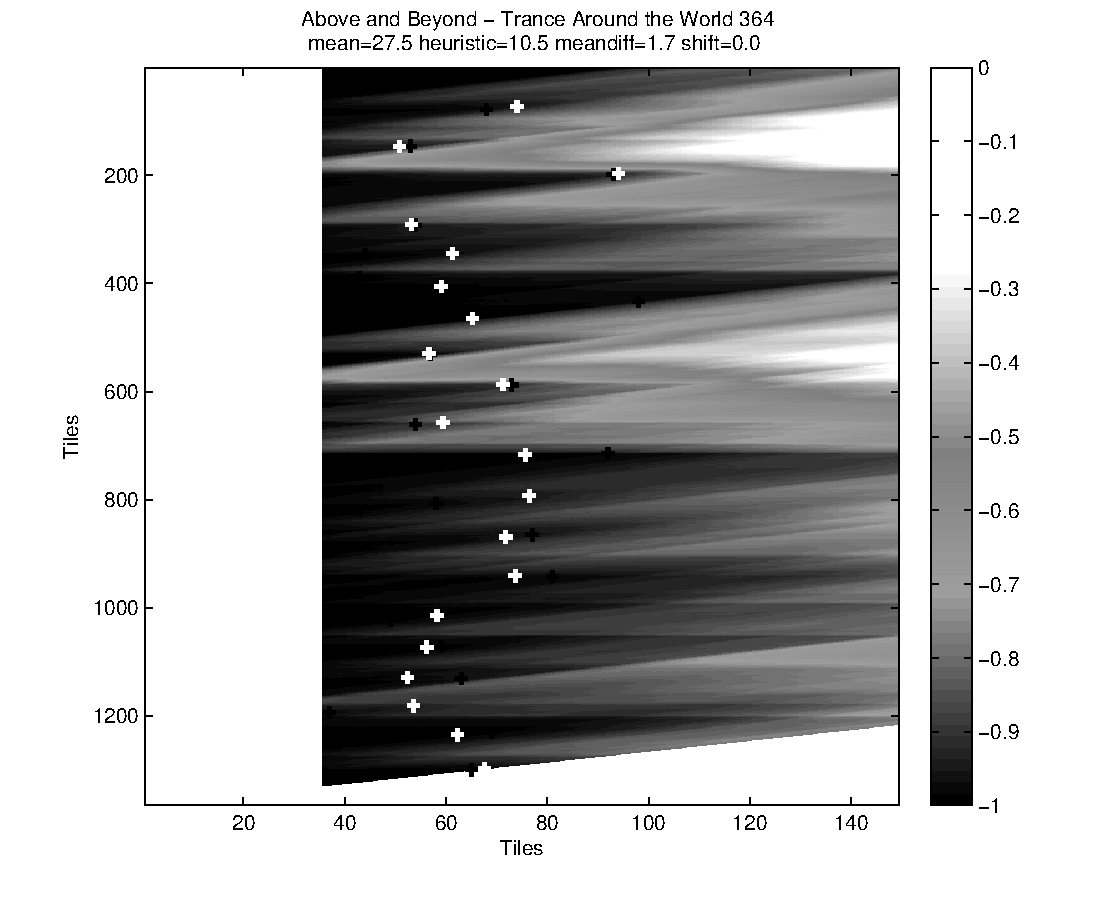
\includegraphics[width=0.45\textwidth]{images/cmsumib1}
			\caption{Summation cost matrices for Magic Island episode 110 with an incentive bias $\Omega=0$ and therefore containing incentives. }
			\label{fig:cmsumib1}
		\end{figure} 
		
		
	
	
	\section{Computing Best Segmentation}\label{best_cost}
	
	We obtain the cost of a full segmentation by summing the costs of its tracks. The goal is now to efficiently compute the segmentation of least cost.
	
	We want to reconstruct $m$ track boundaries ($m+1$ tracks).
	
	A sequence $\t = (t_1, \ldots, t_{m+1})$ is called an $m/T$-segmentation if and only if
	\[
	1 = t_1 < \ldots < t_m < t_{m+1} = T+1.
	\]
	$m$ is the number of tracks we are trying to find and is a parameter of the algorithm. We use the interpretation that track $i \in \{1, \ldots, m\}$ comprises times $\{t_i, \ldots, t_{i+1}-1\}$. Let $\segs^T_m$ be the set of all $m/T$-segmentations. Note that there are a very large number of possible segmentations 
	\begin{multline*}
		|\segs^T_m| ~=~ \binom{T-1}{m-1}
		= \frac{(T-1)!}{(m-1)!(T-m)!} =\\
		\frac{(T-1)(T-2)\cdots(T-m+1)}{(m-1)!} \ge \left( \frac{T}{m}\right)^{m-1}.
	\end{multline*} 
	For large values of $T$, considering all possible segmentations using brute force is infeasible. For example, a two hour long show with $25$ tracks would have more than 
	\[
	\left( \frac{60^2 \times 2}{25}\right)^{24}  \approx 1.06 \cdot 10^{59}
	\] possible segmentations. 
	
	We can reduce this number slightly by imposing upper and lower bounds on the song length.  Recall that $W$ is the upper bound (in seconds) of the song length, $w$ the lower bound (in seconds) and $m$ the number of tracks. With the track length restriction in place, the number of possible segmentations is still massive. A number now on the order of $10^{56}$ for a two hour show with $25$ tracks, $w=190$ and $W=60\cdot15$.
	
	Let $N(T,W,w,m)$ be the number of segmentations with time $T$ (in tiles),
	
	We can write the recursive relation $$N(T,W,w,m) = \sum N(t_m-1,W,w,m-1),$$ where the sum is taken over $t_m$ such that 
	\begin{align*}
		t_m &\le T-w+1 & t_m &\ge T-W+1\\
		t_m &\ge (m-1)w+1 & t_m &\le (m-1)W+1
	\end{align*}
	
	The first two inequalities mean that the length of the last track is within an acceptable boundary between $w$ and $W$. The last two inequalities mean that the lengths of the first $m-1$ tracks are within the same boundaries. 
	
	We calculated the value of $N(7000,60\cdot15,190,25)$ and got $5.20 \cdot 10^{56}$ which is still infeasible to compute with brute force.
	
	Our solution to this problem is to find a dynamic programming recursion.
	
	The loss of an $m/T$-segmentation $\t$ is 
	\[
	\loss(\t) 
	~=~
	\sum_{i=1}^m C(t_i, t_{i+1}-1)
	\]
	We want to compute
	\[
	\best^T_m ~=~ \min_{\t \in \segs^T_m} \loss(\t)
	\]
	To this end, we write the recurrence
	\begin{equation*}
		\best^t_1 ~=~ C(1, t) 
	\end{equation*}
	and for $i\ge2$
\begin{align*}
		\best^t_i ~=~& \min_{\t \in \segs^t_i} \loss(\t)  \\
		~=~& \min_{t_i} \min_{\t \in \segs^{t_i-1}_{i-1}} \loss(\t) + C(t_i, t)  \\
		~=~&  	\min_{t_i} C(t_i, t) + \min_{\t \in \segs^{t_i-1}_{i-1}} \loss(\t)  \\ 
		~=~& \min_{t_i} C(t_i, t) + \best^{t_i-1}_{i-1} \\
\end{align*}
	%On page 7: t_i should range from t-W to t-w. It is about the position of the /last/ song.
	
	In this formula $t_i$ ranges from $t-W$ to $t-w$. We have $T \times m$ values of $\best^T_m$ and calculating each takes at most $O(W)$ steps. The total time complexity is $O(TWm)$.
	
\section{Confidence Intervals}\label{sec:confidence-intervals}
	
It may be useful for some applications to build a framework to allow confidence intervals for our predicted indices. This may also be useful for meaningful comparison of cost matrices.
	
	\subsection{Posterior Marginal of Song Boundary}
	Fix a learning rate $\eta$, and fix $T$ and $m$. Let
	\[
	P(j,s) ~=~ 
	\frac{\displaystyle
		\sum_{\t \in \segs^T_m : t_j = s} e^{- \eta \loss(\t)}
	}{\displaystyle
	\sum_{\t \in \segs^T_m} e^{- \eta \loss(\t)}
}
\]
That is, $P(j,s)$ is the ``posterior probability'' that song $j$ starts at time $s$.

To compute $P(j,s)$, we need an extended notion of segmentation. We call $\t$ a $m/F: T$ segmentation if
\[
F = t_1 < \ldots < t_m < t_{m+1} = T+1.
\]
Let $\segs^{F : T}_m$ be the set of all $m/F-T$-segmentations. 
%
We have
\begin{multline*}
	\sum_{\t \in \segs^T_m : t_j = s} e^{- \eta \loss(\t)}
	~=~
	\sum_{\substack{\t \in \segs^{s-1}_{j-1},\\ 
			\t'\in \segs^{s : T}_{m-j+1}}} 
	e^{- \eta (\loss(\t) +\loss(\t'))}
	~=~ \\
	\left(\sum_{\t \in \segs^{s-1}_{j-1}} e^{- \eta \loss(\t)}\right)
	\left(\sum_{\t \in \segs^{s : T}_{m-j+1}} e^{- \eta \loss(\t)}\right)
\end{multline*}
%
which upon abbreviating
\begin{align*}
	\head^t_m & ~=~ \sum_{\t \in \segs^{t}_{m}} e^{- \eta \loss(\t)} &
	\tail^f_m & ~=~ \sum_{\t \in \segs^{f : T}_m} e^{- \eta \loss(\t)}
\end{align*}
means that we can write
\[
P(j,s) ~=~ \frac{\head^{s-1}_{j-1} \cdot \tail^{s}_{m-j+1}}{\head^T_m}
.
\]
So it suffices to compute $\head^{t}_{m}$ and $\tail^{t}_{m}$ for all relevant $t$ and $m$. We use
\begin{align*}
	\head^t_1 &~=~ e^{-\eta C(1,t)} &
	\tail^f_1 &~=~ e^{- \eta C(f, T-f+1)}
\end{align*}
and for $m\ge2$
\begin{align*}
	\head^t_m 
	&~=~ 
	\sum_{t_m} \sum_{\t \in \segs^{t_m-1}_{m-1}} e^{- \eta (\loss(\t) + C(t_m, t-t_m+1))} 
	\\
	&~=~ 
	\sum_{t_m} e^{-\eta C(t_m, t-t_m+1)} \sum_{\t \in \segs^{t_m-1}_{m-1}} e^{- \eta \loss(\t)}
	\\
	&~=~ 
	\sum_{t_m} e^{-\eta C(t_m, t-t_m+1)} \head^{t_m-1}_{m-1}
	\\
	\tail^f_m 
	&~=~ 
	\sum_{t_2} \sum_{\t \in \segs^{t_2 : T}_{m-1}} e^{- \eta (C(f, t_2-f)
		+ \loss(\t))}\\
	&~=~
	\sum_{t_2} e^{- \eta C(f, t_2-f)} \sum_{\t \in \segs^{t_2 : T}_{m-1}} e^{- \eta \loss(\t)}\\
	&~=~
	\sum_{t_2} e^{- \eta C(f, t_2-f)} \tail^{t_2}_{m-1}\\
\end{align*}

\begin{figure}
	\centering
	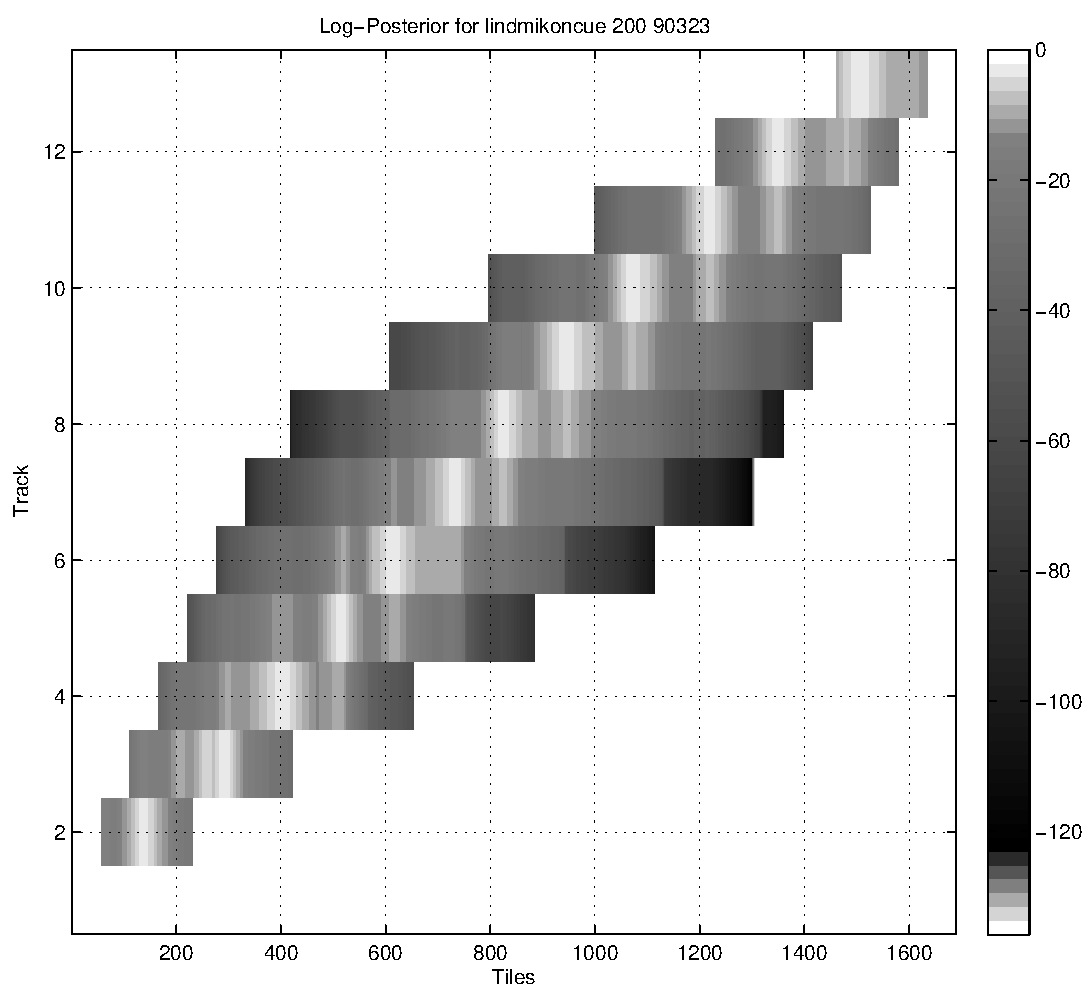
\includegraphics[width=0.5\textwidth]{images/posterior2}

	\bigskip

	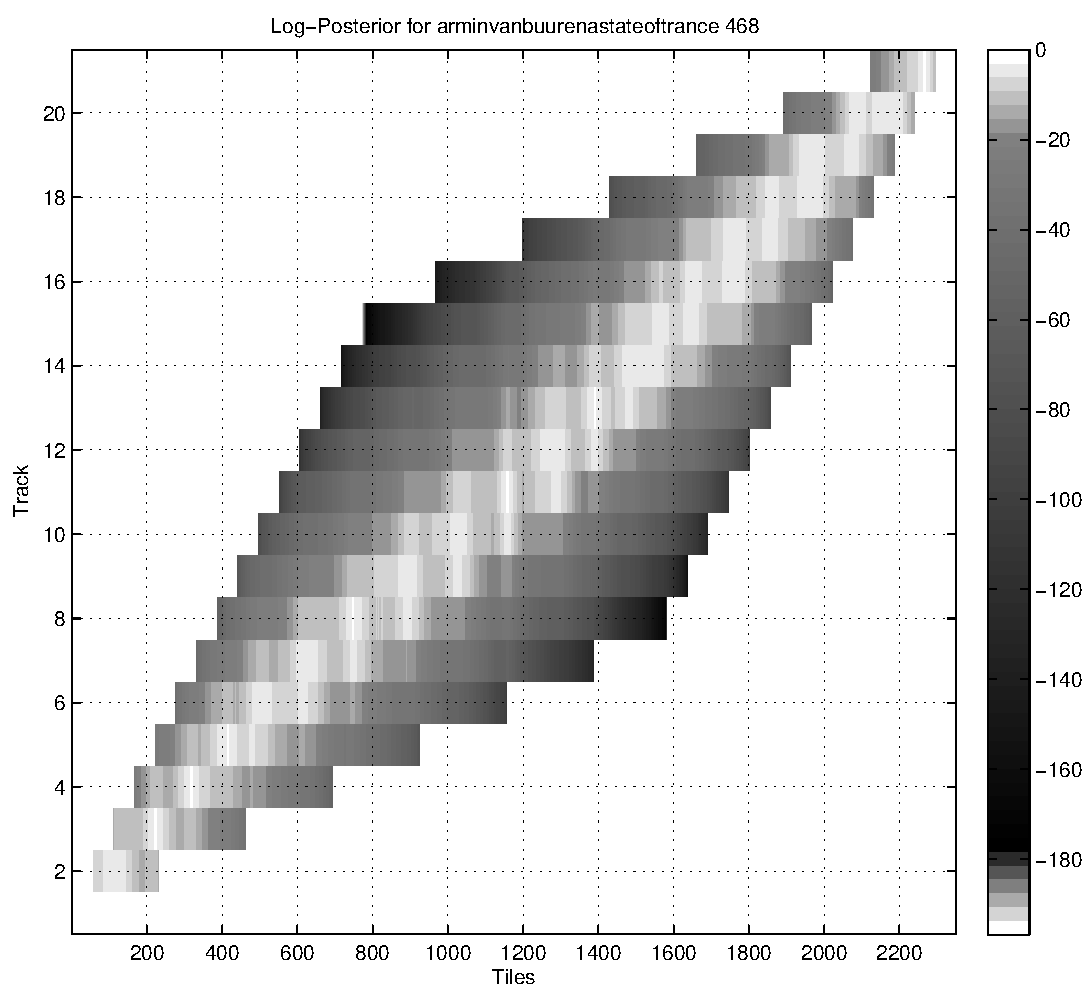
\includegraphics[width=0.5\textwidth]{images/posterior3}
	\caption{A visualization of $log(P(j,s))$ ($\eta=10$) for one of the shows in the test set using the cost matrix parameters from experiment $10$. The actual tracks are overlaid as white crosses.}
	\label{fig:posterior3}
\end{figure} 

See Figure~\ref{fig:posterior2} for an example of the posterior for a radio show. 

\subsection{Posterior Marginal of Song Position}
Fix a learning rate $\eta$, and fix $T$ and $m$. Let
\[
P(j,s,f) ~=~ 
\frac{\displaystyle
	\sum_{\t \in \segs^T_m : t_j = s \land t_{j+1}-1 = f} e^{- \eta \loss(\t)}
}{\displaystyle
\sum_{\t \in \segs^T_m} e^{- \eta \loss(\t)}
}
\]
That is, $P(j,s,f)$ is the ``posterior probability'' that song $j$ starts at time $s$ and finishes at time $f$.
%
In the same vein as the last section, we now get
\[
P(j,s,f) ~=~ \frac{\head^{s-1}_{j-1} \cdot e^{-\eta C(s, f-s+1)} \cdot \tail^{f+1}_{m-j}}{\head^T_m}.
\]


\subsection{Track Index Confidence}

We can use the posterior marginal of song boundary to give estimates of confidence on track index placement and time accuracy.

To estimate the uncertainty of correct track alignment, we select the next highest probability of other track placements at the same time of the optimal placement from $P(j,s)$ and normalize them by the probability of the optimal placement.

Let track index confidence
\begin{align*}
I( j ) = 1-\frac{ P( \{1,\ldots,M\} \setminus j, \mathrm{SortInd}( P(j, 1,\ldots,T)_1)^2 }{ \max( P(j, 1,\ldots,T)_2) }
\end{align*}

where $\mathrm{SortInd}(l)$ will return the original indices corresponding to the sorted list of $l$. 

\subsection{Track Time Confidence}

Track time uncertainty is estimated by normalizing the value of the next most significant peak in $P(j,\forall s)$ by the probability of actual track placement (which is the most significant peak). 
Let 
\begin{align*}
\tilde I( j ) = 1-\frac{ \mathrm{Peaks}( P(j, 1,\ldots,T ) )_2 } { \mathrm{Peaks}( P(j, 1,\ldots,T ))_1 }
\end{align*} where $Peaks(s_i)$ is a peak finding algorithm that returns the peaks in descending order of magnitude (we used the \texttt{findpeaks} function in MatLab).


\section{Experiments}

\subsection{Training Set}

We selected $6$ shows at random (two of each show type)  to create a training set, which we will refer to as the \textit{GitHub training set}. See Table~\ref{table:githubset} to see the shows we selected.

\begin{table*}[t]
	
	\centering
	\caption{The shows randomly selected for inclusion in the \textit{GitHub training set}.}
	\label{table:githubset}
	
	\begin{tabular}{llll}
		\#         & \textbf{Show Name}          & \textbf{Artist}  & \textbf{Date Broadcast} \\
		\textbf{1} & A State Of Trance 453       & Armin Van Buuren & April 2010              \\
		\textbf{2} & A State Of Trance 462       & Armin Van Buuren & June 2010               \\
		\textbf{3} & Magic Island 098            & Roger Shah       & March 2010              \\
		\textbf{4} & Magic Island 112            & Roger Shah       & July 2010               \\
		\textbf{5} & Trance Around The World 364 & Above \& Beyond  & March 2011              \\
		\textbf{6} & Trance Around The World 372 & Above \& Beyond  & May 2011               
	\end{tabular}
	
\end{table*}

\subsection{Finding The Best Cost Matrix}\label{sec:findingbestcostmatrix}

We used the GitHub training set to develop the cost matrices from first principles and to find robust parameters using a genetic algorithm search.



In our experiments we decided to fix the tile size at $5$ seconds for the sake of speed. A lower tile size does increase accuracy but only marginally. Higher tile sizes can perform more robustly (fewer catastrophic misalignments) but progressively lose out on accuracy.







% GENETIC ALGORITHM DESCRIPTION
\section{Estimating Segment Count}\label{sec:trackcount}

The original goal of our work was providing the best possible segmentation given a fixed number of tracks $m$, rather than estimating $m$. The problem domain is reasonably unique; the number of segments is known a priori but segmentation itself is not.

In the most basic setting. The number of tracks could be estimated as the variable of track lengths is Gaussian (see Figure~\ref{fig:tracklengths}). 

We propose the following method of adapting our framework to estimate the number of contiguous segments in a data stream. 

	\begin{figure}
		\centering
		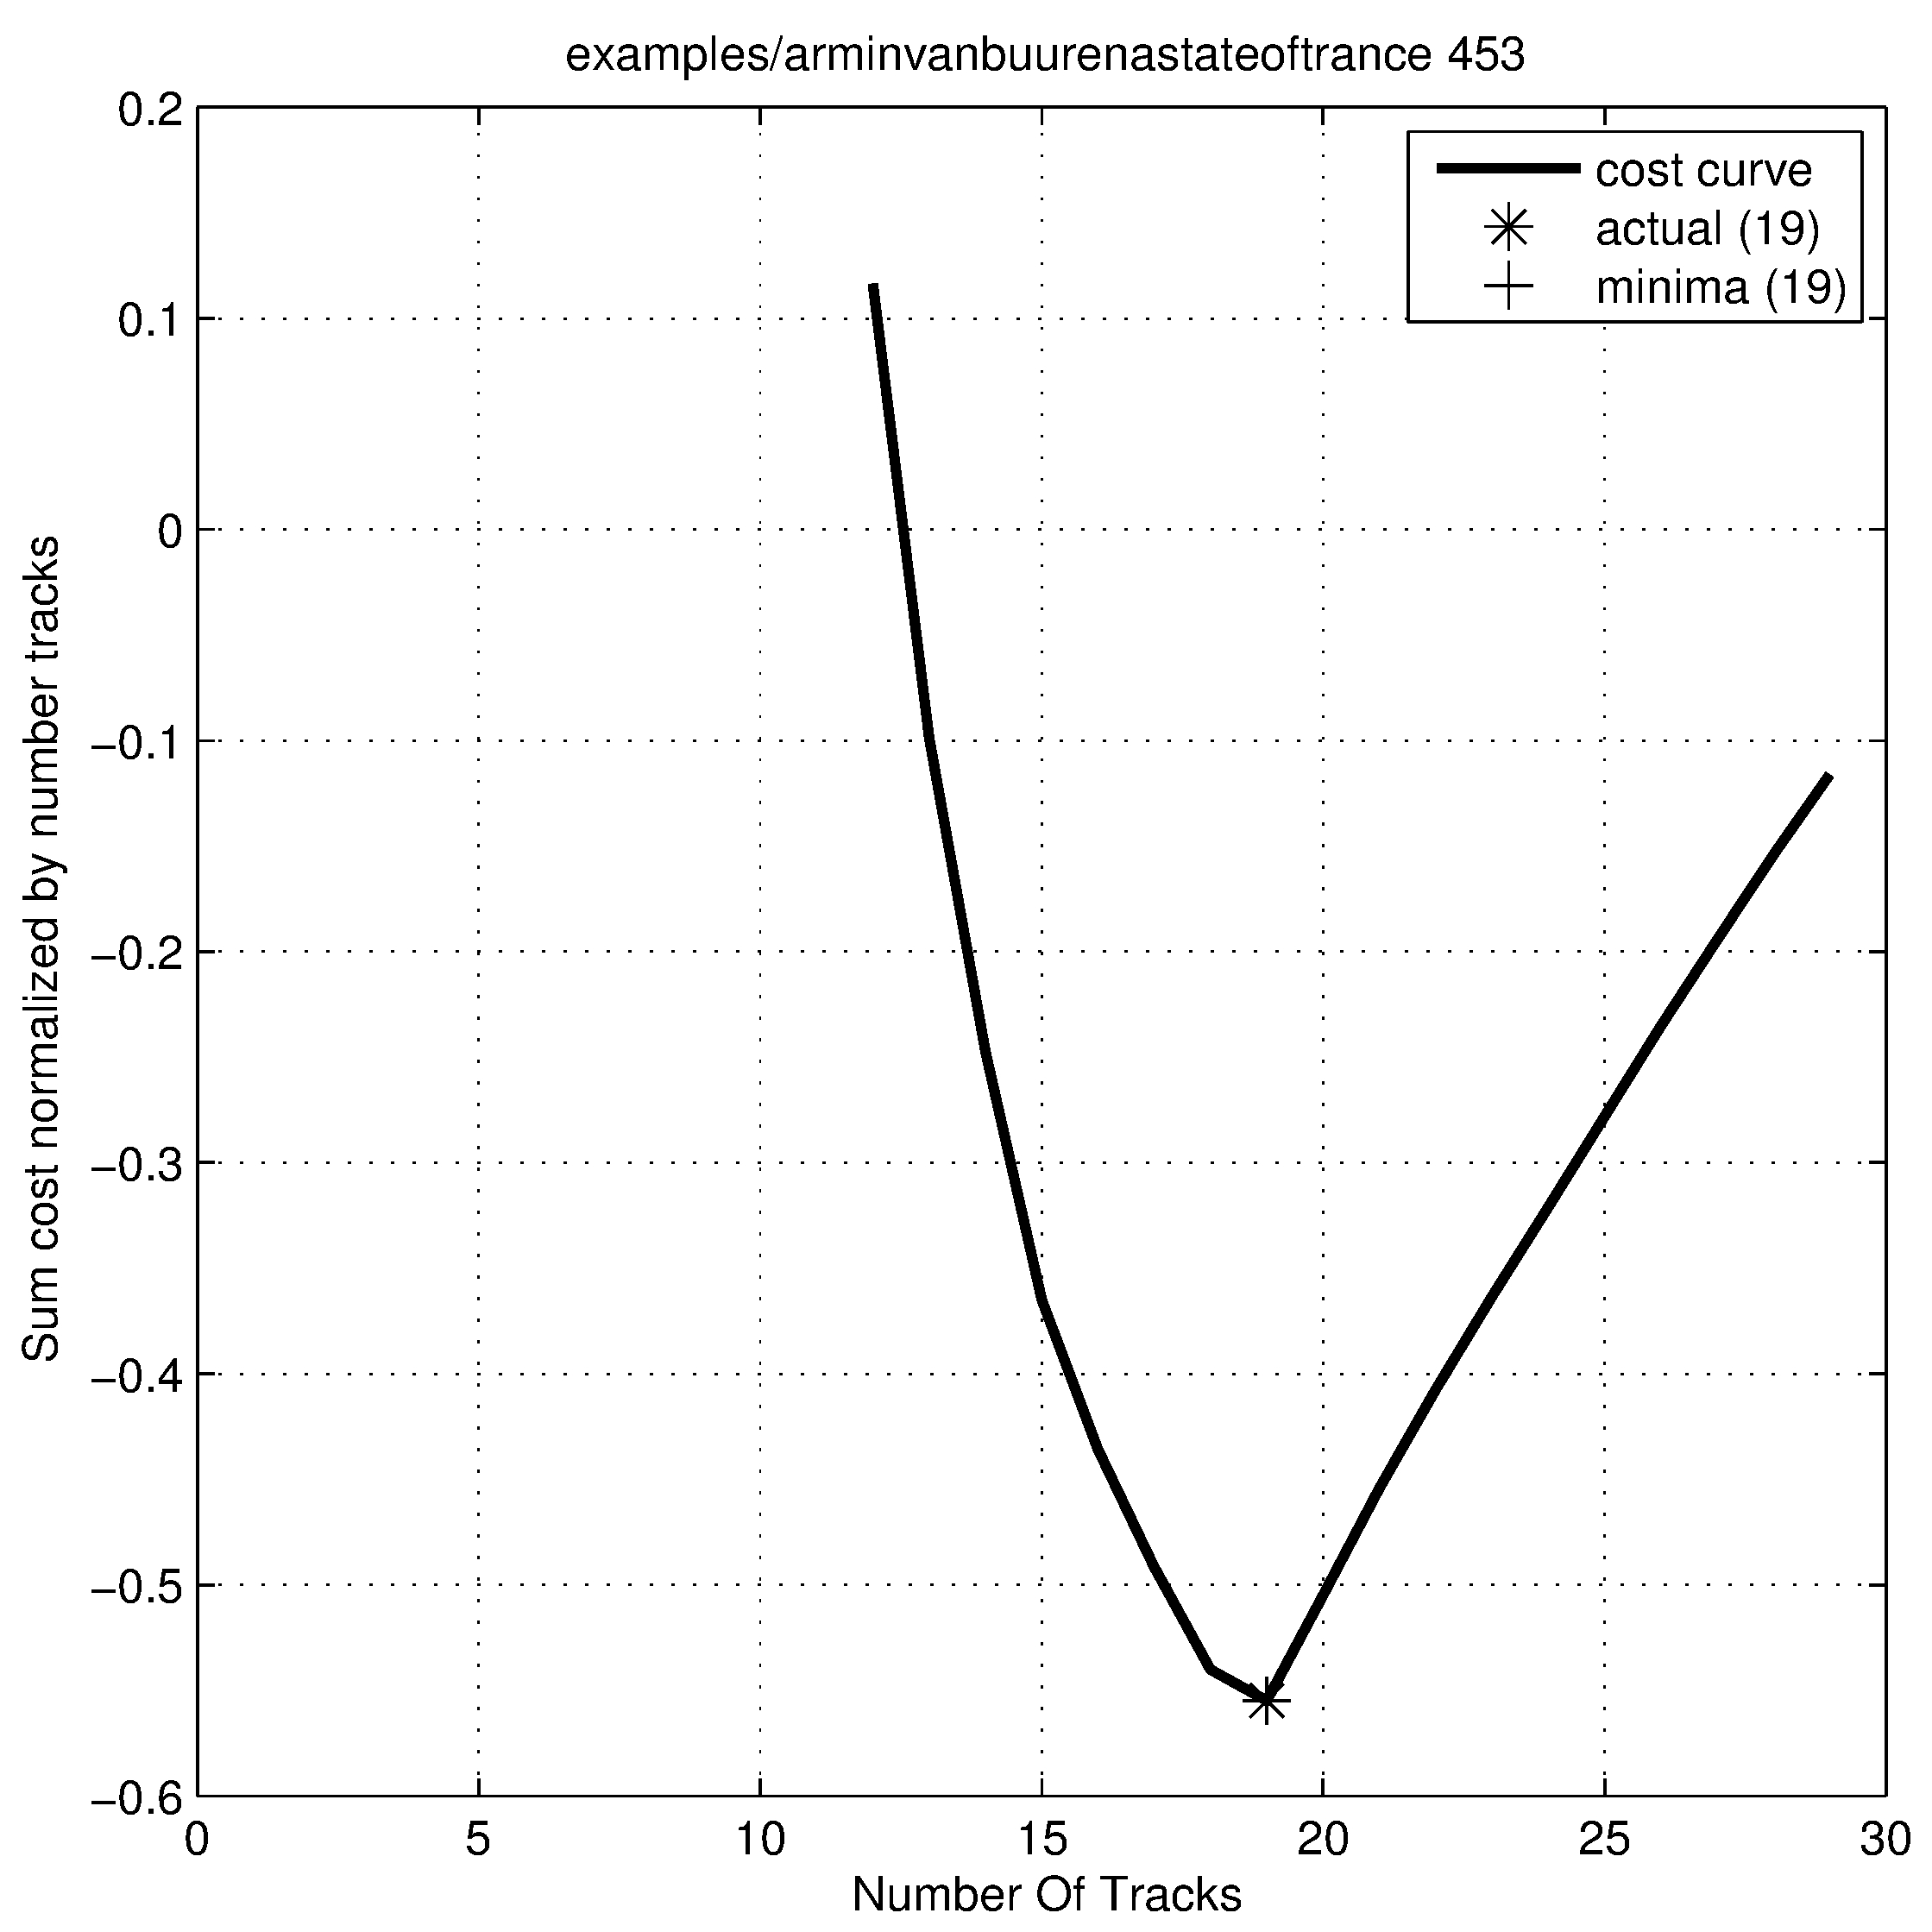
\includegraphics[width=0.5\textwidth]{images/trackestimate}
		\caption{Number of tracks estimated correctly a show in the GitHub training set after a genetics algorithm was run to select a new set of configuration parameters.}
		\label{fig:github_trackestimation}
	\end{figure}

	\begin{figure}
		\centering
		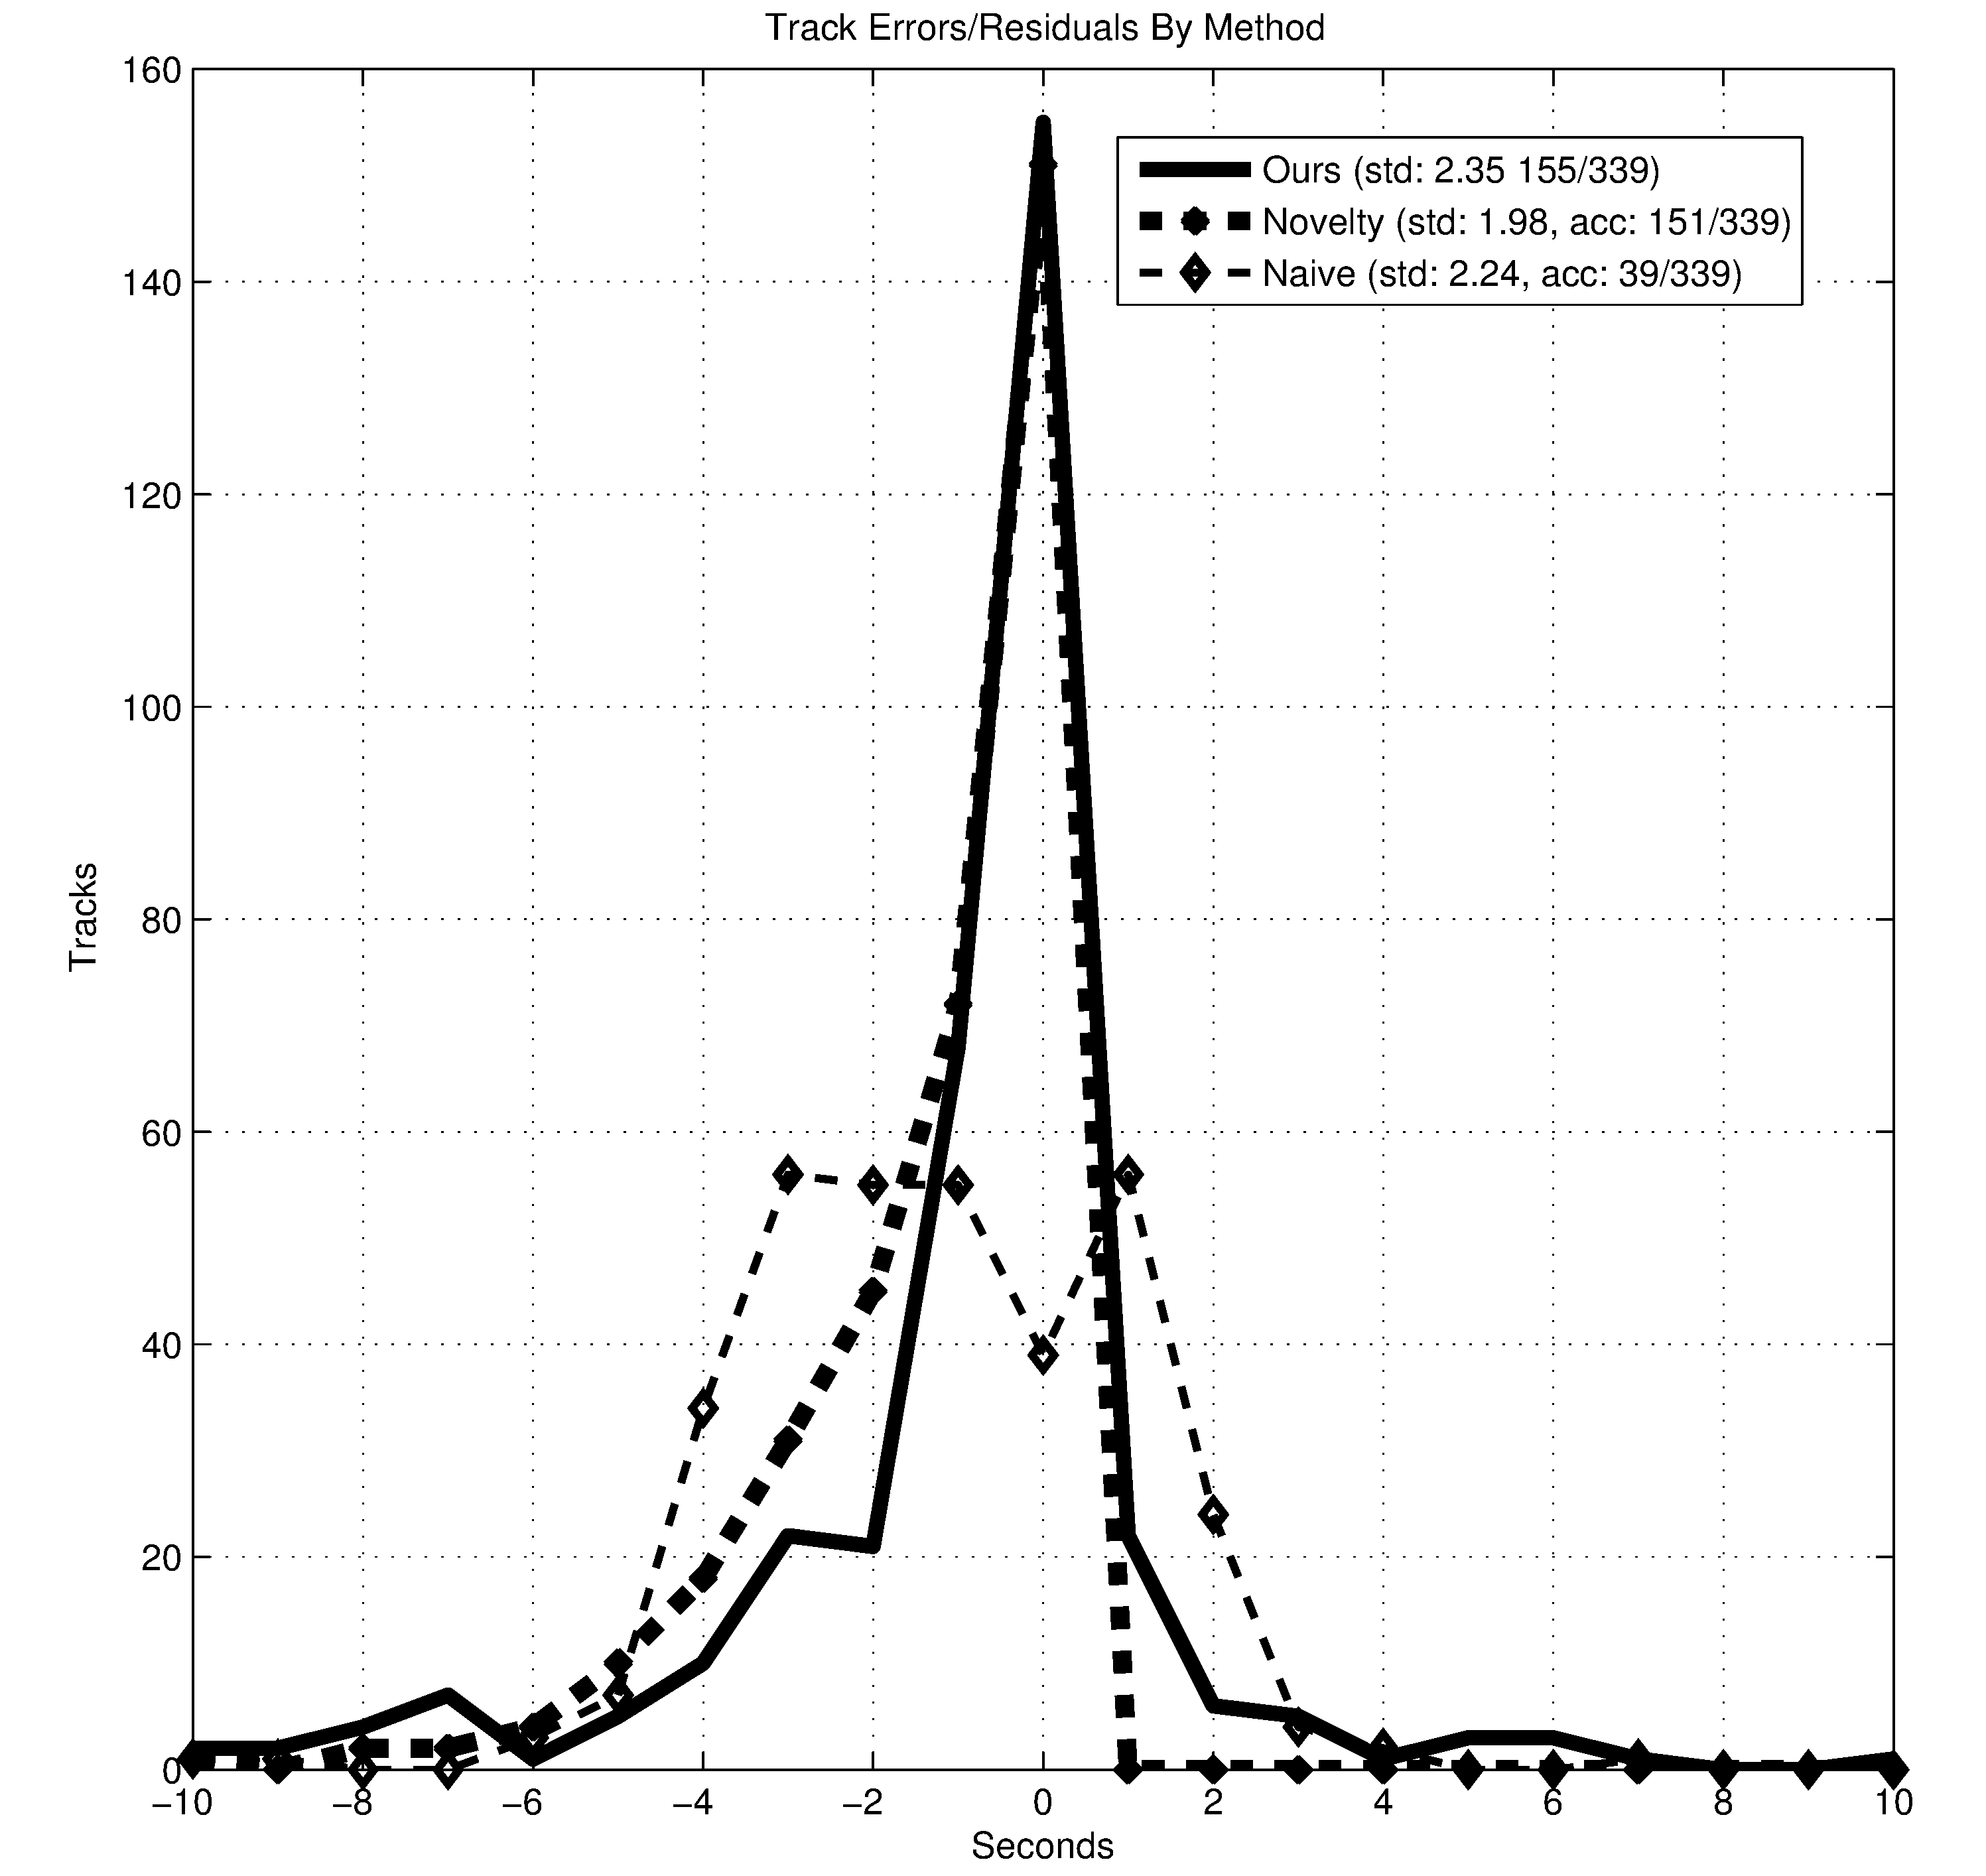
\includegraphics[width=0.5\textwidth]{images/trackshift}
		\caption{}
		\label{fig:track_shift}
	\end{figure}

\section{Evaluation}\label{eval_crit}

It is challenging to quantify the performance of our method because if we misplace any tracks, it may have a cascade effect. For example if we place one track too many early on in a show, many of the subsequent tracks may be correctly detected but placed out of alignment. 

For the task of computing the best cost segmentation when the number of tracks are known a priori, we can use simple statistical descriptions of the track residuals $|P_{st}-A_{st}|$ where $P$ is the predicted track, $A$ the actual track, for show $s$ and track $t$ (for all $s$ and $t$ in the corpus). The mean average will give a good indication of the accuracy combined with the amount of misplacements. The median of the residuals will indicate the actual track accuracy invariant to any catastrophic misplacements. The standard deviation of the residuals will indicate the spread of error. 

\section{Results}\label{sec:results}

Please see Table~\ref{tab:results} for the main table of results, Figure~\ref{fig:shifthistogram} for a histogram of predicted versus actual differences for experiment $10$. 



\begin{tabular}{|c|c|c|c|c|c|}
	\hline 321 & 321 &  & dsa &  &  \\ 
	\hline 312 & 312 & dsa & dsa &  &  \\ 
	\hline  &  &  & d & dasd &  \\ 
	\hline  &  &  & asdas & dsa &  \\ 
	\hline  &  &  &  &  &  \\ 
	\hline 
\end{tabular} 

	\begin{figure}
		\centering
		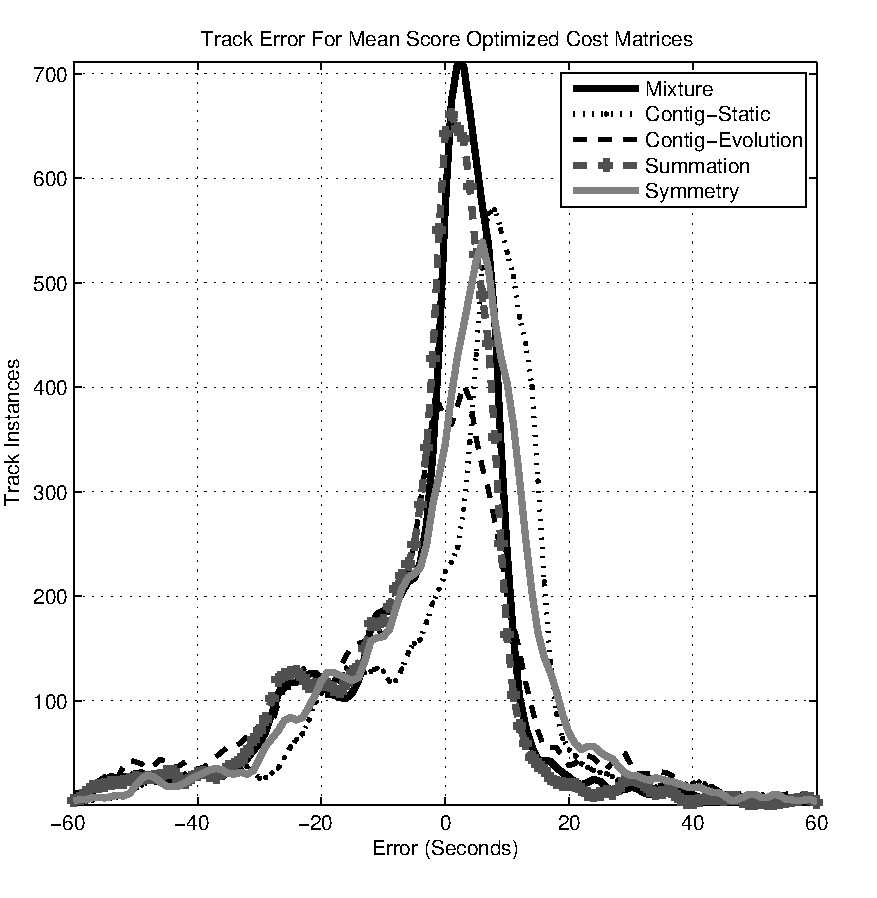
\includegraphics[width=0.5\textwidth]{images/shift_histogram}
		\caption{Histogram of the residuals (errors) between reconstructed and human captured time indices. Apart from obvious noise there appears to be a tendency for the algorithm to place an index slightly earlier. Contig-static cost matrix apparently contained parameters selected through optimization that shifted it to remove some of this effect.    }
		\label{fig:shifthistogram}
	\end{figure} 


On our previous work we were using a disincentive only summation matrix, and found that normalizing it on the square root of the width produced the best result. This would have been necessary to encourage placement of longer tracks as no incentive was present. So experiment $11$ is roughly comparable and indeed produces the same overall mean average to that previous experiment ($\approx 20$S). Note that we no longer discard any shows from evaluation which makes the result stronger. 


\begin{figure*}
	\begin{center}
		
	
	
		
		\begin{minipage}[t]{0.45\linewidth}
			\begin{center}
				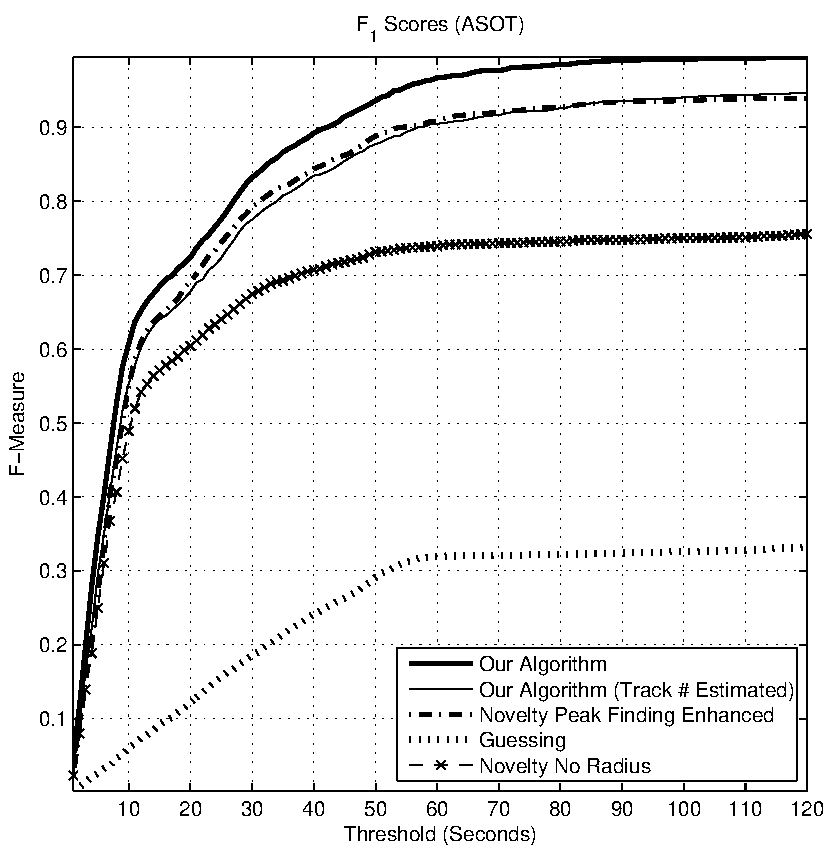
\includegraphics[scale=0.5]{images/fscores/fasot}
			\end{center}
		\end{minipage}
		\begin{minipage}[t]{0.45\linewidth}
			\begin{center}
				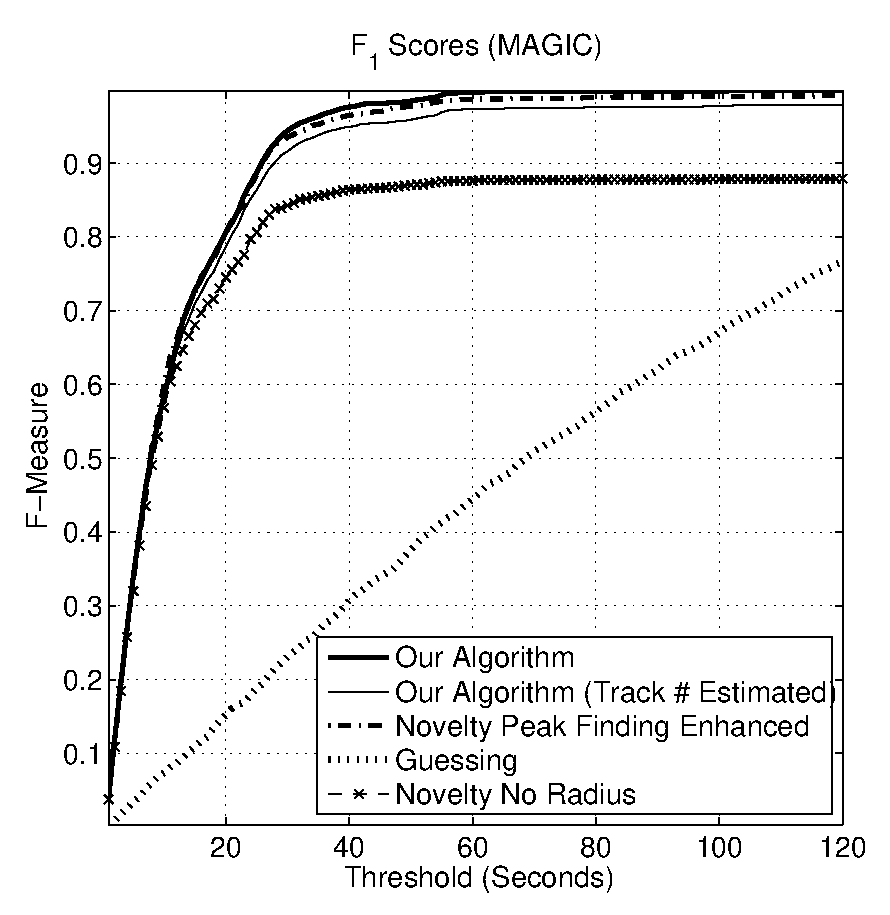
\includegraphics[scale=0.5]{images/fscores/magic}
			\end{center}
		\end{minipage}
		\bigskip
		
		\begin{minipage}[t]{0.45\linewidth}
			\begin{center}
				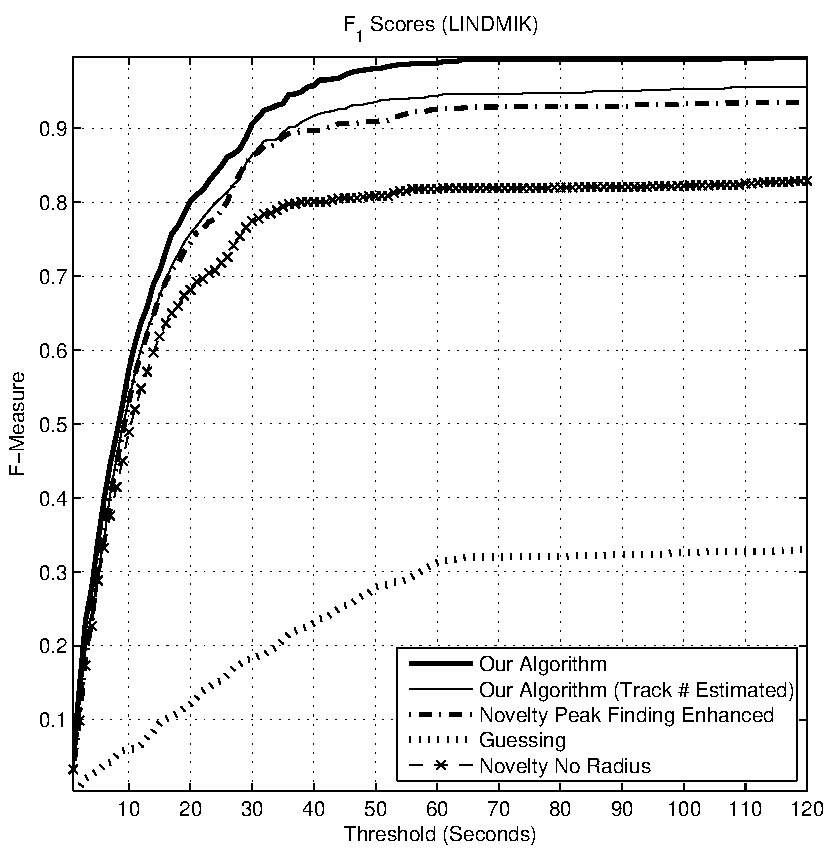
\includegraphics[scale=0.5]{images/fscores/lindmik}
			\end{center}
		\end{minipage}
		\begin{minipage}[t]{0.45\linewidth}
			\begin{center}
				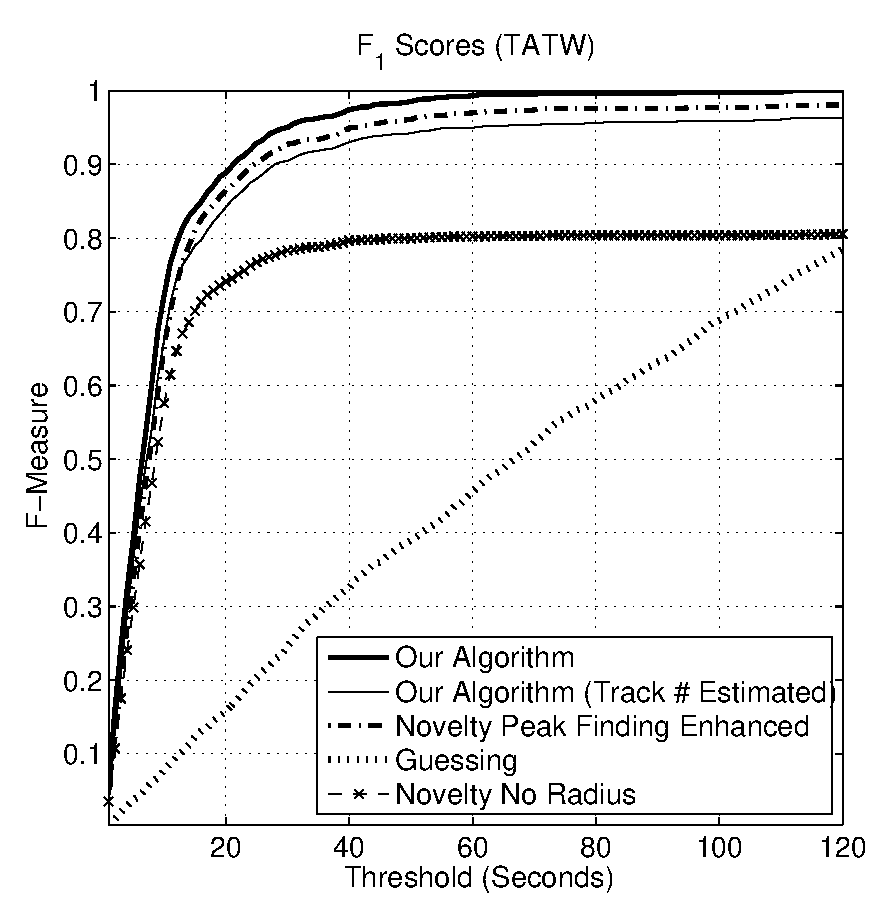
\includegraphics[scale=0.5]{images/fscores/tatw}
			\end{center}
		\end{minipage}
		
	\end{center}
	
	\caption{lalala}
	\label{fig:fscores_breakdown}
		
\end{figure*}


\begin{figure}
	
		\begin{center}
			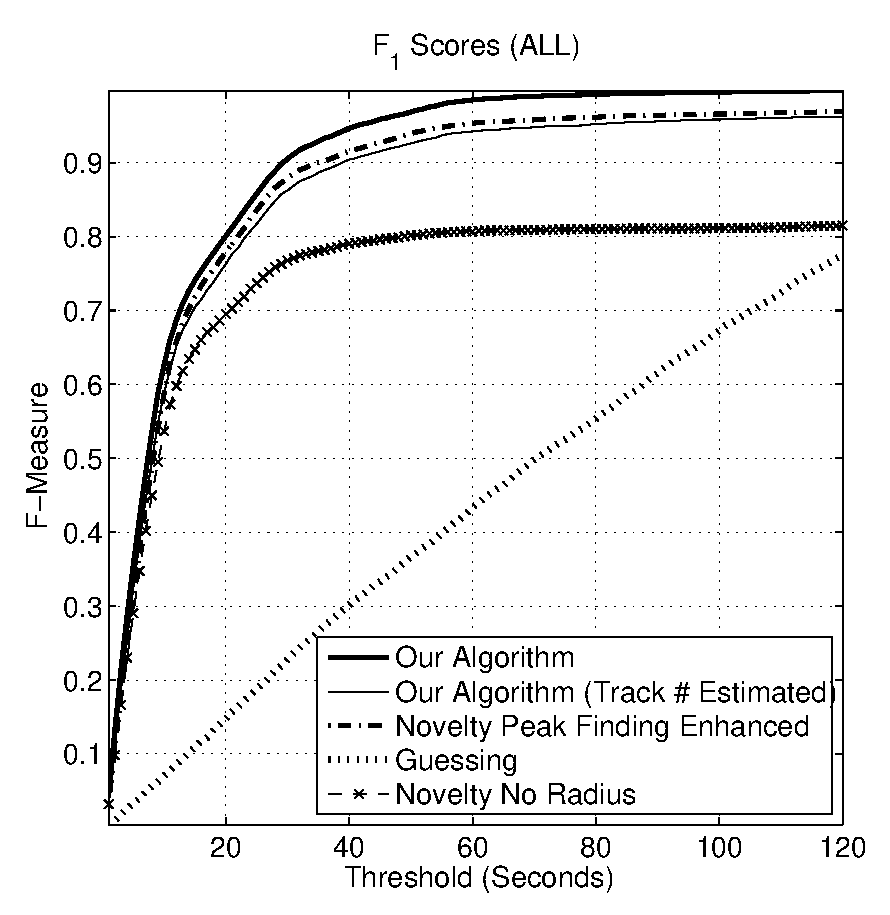
\includegraphics[scale=0.5]{images/fscores/fall}
		\end{center}

	
	\caption{Comparison between our algorithm and the Foote novelty peak finding approach on all of the datasets.}
	\label{fig:fscores_best}
	
\end{figure}

\section{Summary}\label{conclusions}

We believe our algorithm would be useful for segmenting DJ-mixed audio streams in batch mode. It would be excellent if Sound Cloud\footnote{\url{http://www.soundcloud.com}} for example started to do something similar. Sound Cloud is an on-line music service with many electronic dance music radio shows with the track listing in text. This method would allow them to reliably segment the shows, and they could display an interactive segmentation in the music player. 

The new cost matrices in combination improve robustness significantly over single matrices or regularised single matrices (as in our last paper). We are seeing about a 50\% improvement in overall mean accuracy over single cost matrices that are correctly normalized. The new cost matrices improve on many drawbacks of our previous work (mainly that it was vulnerable to dissimilar regions within tracks). 

%bit weak
Our method still has one key drawback that we are aware of. This is the rare instance where there are head or tail segments to a track that seem independent from the rest of the track. When these are small they usually get absorbed without any problems but they can cause misplacements. In spite of this issue we suspect that our predictions are more accurate and more consistent than the human equivalents while not being as precise in situations when our index agrees with theirs.

A more precise corpus where the DJ was also the cuesheet author would allow us to tune the parameters more succinctly and also the generation of an artificial dataset to test against. This work is forthcoming. 

%TODO We want to do an online version


%TODO
We would also like to implement some of the methods in the literature (which were mostly designed for scene analysis) to see if we outperform them. It would be tricky to get an exact comparison because we could not find an unsupervised deterministic algorithm which finds a fixed number of strictly contiguous clusters. We could however adapt existing algorithms to get a like for like comparison. 



\section{Acknowledgements}\label{sec:acknowledgements}

We would like to thank Mikael Lindgren and Denis Goncharov from cuenation\footnote{\url{http://www.cuenation.com}} for their help explaining how they make cue-sheets and for providing the data set to test the algorithm on.

\section{Materials}\label{sec:materials}

All the code presented in this paper with the training set is available on GitHub \footnote{\url{github.com/ecsplendid/DanceMusicSegmentation}}. The large data set ($\approx130$GB) we received from Denis Goncharov and Mikael Lindgren can easily be made available on request (it is in a cloud storage account).


\bibliographystyle{ieeetr}
\bibliography{bib/references,bib/refs}

\end{document}
